\documentclass[12pt]{article}
\usepackage[utf8]{inputenc}
\usepackage[english]{babel}

% amsmath package, useful for mathematical formulas
\usepackage{amsmath}
% amssymb package, useful for mathematical symbols
\usepackage{amssymb}
% more beautiful fraction signs
\usepackage{nicefrac}

% line numbering
% \usepackage{lineno}

% hyperref
\usepackage[hidelinks]{hyperref}

% graphicx package, useful for including eps and pdf graphics
% include graphics with the command \includegraphics
\usepackage{graphicx}

% cite package, to clean up citations in the main text. Do not remove.
\usepackage{cite}
\usepackage{color} 
\usepackage{upgreek}%non-italic greek letters

% Use doublespacing - comment out for single spacing
\usepackage{setspace} 
\usepackage{mathtools}%\prescript
\doublespacing


% Text layout
\topmargin 0.0cm
\oddsidemargin 0.5cm
\evensidemargin 0.5cm
\textwidth 16cm 
\textheight 21cm

% Bold the 'Figure #' in the caption and separate it with a period
% Captions will be left justified
%\usepackage[labelfont=bf,labelsep=period,justification=raggedright]{caption}

\bibliographystyle{plain}

\newcommand{\parc}[2]{\frac{\partial #1}{\partial #2}}
\newcommand{\bsym}[1]{\ensuremath{\boldsymbol{#1}}}


% Leave date blank
\date{}

\pagestyle{myheadings}

%% PLEASE INCLUDE ALL MACROS BELOW

%% END MACROS SECTION

\begin{document}

% Title must be 150 characters or less
\begin{flushleft}
{\Large
\textbf{Novel limiting Criterion for Discontinuous Galerkin Method Applied in Shallow Water Equations}
}
% Insert Author names, affiliations and corresponding author email.
\\

Martin Fi\v{s}er$^{1,\ast}$, Ilhan \"Ozgen-Xian$^2$, Adri\'an
Navas-Montilla$^3$, (add other authors as fit)


$^1$NTIS - New Technologies for the Information Society, Faculty of
Applied Sciences, University of West Bohemia, Pilsen, Czech Republic

$^2$EESA, Lawrence Berkeley National Laboratory, Berkeley, California,
USA

$^3$Centro Universitario de la Defensa, Universidad de Zaragoza,
Zaragoza, Arag\'on, Spain

$^\ast$E-mail: martin.fischer1415@gmail.com
\end{flushleft}

%\linenumbers

\section*{Abstract} 

This paper presents a third-order discontinuous Galerkin method for
the shallow water equations with a novel limiting method to ensure
stability.  This method limits the solution in so-called ``troubled
cells'', which are detected based on the shape of the approximating
functions.  We further present a numerical treatment of wet/dry
interfaces to ensure positive water depths.  The well-balanced
property of the scheme is preserved through the surface gradient
method.  The scheme is compared with analytical solutions in several
computational test cases to verify its properties.

\section*{Keywords}

shallow water equations, wet/dry interface, HLL scheme, uneven bed,
discontinuous Galerkin method, limiting process, bed slope source term

\section{Introduction}

The study and prediction of environmental and geophysical flow
processes requires knowledge of the spatially and temporally varying
flow field.  Large scale, predominantly horizontal flow fields in such
application fields are usually computed through the numerical solution
of the depth-integrated shallow water equations (SWE).  For example,
SWE-based models are used for tsunami and coastal inundation
predictions in \cite{Marras:2016, Vater2019, Qin:2019}, flood
predictions \cite{George2011, Echeverribar2019}, and river hydraulics
\cite{Persi:2019}.  More recently, the SWE have been used in
rainfall-runoff studies in small natural catchments \cite{Mugler2011,
  Lacasta2014, Simons2014, Xia2019, CaviedesVoullieme2020}.

Many of the aforementioned SWE applications involve wetting and drying
processes.  For example, coastal simulations involve wave runup and
overtopping \cite{Vater20151, Medeiros2013, Vater2019}. In
rainfall-runoff simulations, cells frequently dry out and get flooded
\cite{Simons2014, Lacasta2014, Xia2017}. Flood simulations feature a
flood front, which switches cells from dry to wet as it propagates
through the domain \cite{George2011}.  The interface between a wet and
a dry cell is usually referred to as a wet/dry interface
\cite{Bollermann2013, Beisiegel2015} and requires special
considerations. TODO: 

The mathematical model of shallow water equations contains the source
terms. The bed slope source term is caused by the bed
irregularities. This source term is well described in many works like
\cite{Ambati2007452,Ambati20071233,kesserwani2015,Beisiegel2015,Tassi2007998}.

The proper numerical treatment of these wet/dry interfaces is
directly related to the crucial properties of (i) mass conservation,
(ii) C-property, (iii) well-balancedness, (iv) positivity-preserving,
and (v) shock-capturing.  In order to ensure an accurate solution, the
numerical scheme must satisfy these properties
\cite{CaviedesVoullieme2020}.

In recent years, discontinuous Galerkin (DG) methods have gained
significant interest as a means to numerically solve the SWE
\cite{CaviedesVoullieme2015, kesserwani2015, Vater20151, Marras:2016,
  Kesserwani2019, Vater2019, CaviedesVoullieme2020,
  NavasMontilla2020}.  The DG method uses a local piecewise-polynomial
representation of the solution, which is driven by fluxes across cell
interfaces.  Thus, the DG method is locally conservative.  Higher
order of accuracy is achieved by increasing the polynomial order.


In most of these cases wetting and drying processes of the cells occur
during the simulation, e.g. part of the computational domain may fall
dry or the domain may start initially dry and get flooded.   In
\cite{Vater20151} the wet/dry interface treatment is described for the
second order DGFEM. In this work the treatment suitable for the third
order DGFEM is suggested.


Except for wet/dry interface and bed slope source term, special
treatment is also needed if the shocks and discontinuities are present
in the computational domain. High order accuracy schemes have to be
limited to prevent them from the appearance of non-physical
oscillations. In the theory of the finite volume method with linear
reconstruction of the conservative variables, some TVD-minmod limiter
restricts the variation of the local slope of the linear approximation
with respect to the upstream and downstream gradients. This is
referred to as a global limiting process. Accordingly to
\cite{krivodonova2004,shu2005} this global limiting approach leads to
the loss of accuracy. Thus the limiter is used only in 'troubled'
cells. In \cite{krivodonova2004} the discontinuity detection scheme
was used to define these cells. The same criterion was used in
\cite{Ambati2007452}. In \cite{kesserwani2015}, Kesserwani added the
criterion of monotonicity of the solution. Disadvantage of the
discontinuity criterion is the definition of the discontinuity
itself. Discontinuity in the solution is compared with a predefined
constant which defines the 'troubled' cells. Unfortunately this
constant can be arbitrarily large and depends on the study case.
Within this work we suggest novel criterion of defining 'troubled'
cells. This criterion is based on the shape of the solution in the
finite element cell and not depends on any constant.

In the 'troubled' cells the limiting process is implemented. In
\cite{JAFFRE1995,Ambati2007452}, the limiting-dissipation operator was
used to limit the numerical solution. Artificial viscosity was used
for example in \cite{cesenek2013, bublik2011,Bublik2015329}. Within
this work, the process described in \cite{Cockburn1989b} is used. The
solution is limited by decreasing of the order of accuracy to the
second order. This second order solution was then limited by minmod
limiter. Finite volume limiters were also adopted in \cite{yang2009}.

The novel criterion of defining 'troubled' cells and wet/dry interface
treatment are tested and validated by the classical benchmarks and
compared by other numerical methods and analytical solutions at the
end of this paper.

\section{Governing Equations}
Depth-averaged one-dimensional shallow water equations can be written in 
conservative form as
\begin{equation}\label{SWE1D}
\parc{\mathbf{W}}{t}+
\parc{\mathbf{F}}{x}=\mathbf{S}_b,
\end{equation}
where \textbf{W} is the vector of conservative variables described by the 
water depth $h$ and flow velocity $u$ as
\begin{equation}\label{konz}
\mathbf{W}=\begin{bmatrix}
h\\
hu\\
\end{bmatrix},
\end{equation}
\textbf{F} is the vector function of inviscid flux
\begin{equation}\label{flux}
\mathbf{F}=\begin{bmatrix}
hu \\ 
hu^2 + \frac{1}{2}g h^2\\
\end{bmatrix},
\end{equation}
here $g$ is gravity acceleration. Bed slope source term $\mathbf{S}_{b}$ is defined as
\begin{equation}\label{Sb}
\mathbf{S}_{b}=\begin{bmatrix}
0 \\
-g h\parc{B(x)}{x}\\
\end{bmatrix},
\end{equation}
where $B(x)$ is the bottom topography. $B(x)$ might vary in time, however 
is considered time-independent in this work.

The source vector may further contain rain source term, bed friction term, fluid viscosity effects, wind shear, turbulent viscosity or Coriolis forces, depending on the case under consideration. These effects are neglected in this work. 

\section{Numerical Scheme of Discontinuous Galerkin Method}\label{NS}
In this section, numerical scheme of DGFEM is describe. However, it is only basic description of the method. More detailed description of the method can be found in \cite{reed1973}. 

If not redefined, the following nomenclature is used in the article. Index $k$ is iterator over the equations in the mathematical model (i.e., $k$ varies from 1 to 2 in case of 1D SWE model). Index $i$ is iterator over the finite elements. Index $p$ iterates over the Gaussian points and indexes $j$ and $l$ iterate over the basis functions.

Let us consider a 1D computational area $\Omega=[a,b] \subset \mathbb{R}$ and let $t\in[0,T]$. Let $\mathcal{T}=\lbrace \Omega_i \rbrace_{i=1}^n$ be the discretization of the computational area where $\Omega_i=[x_{i-\frac12},x_{i+\frac12}]$ satisfies $\Omega_n \cap \Omega_m=\emptyset$ for $m\neq n$ and $\cup_{i}\Omega_i=\Omega$.

The solution of (\ref{SWE1D}) is from the space $\mathbf{S}_h=S_h\oplus S_h$ such that
\begin{equation}
S_h=\lbrace q \in L^2([a,b]):q|_{\Omega_i}\in P^p(\Omega_i),\forall \Omega_i\rbrace
\end{equation}
  here $P^p(\Omega_i)$ is the space of polynomials with degree less than or equal to $p$ in $\Omega_i$. The set $\lbrace \varphi_i^j \rbrace_{j=1}^{n_b}$ is a basis of the space $P^p(\Omega_i)$.

The multiplying of the Equation \ref{SWE1D} by the testing function $\textbf{v}(x)\in \mathbf{S}_h$ and integrating over the finite element $\Omega_i$ yields
\begin{equation}\label{testF}
\int_{\Omega_i}\parc{\mathbf{W}(x,t)}{t} \textbf{v}(x)  \ d\Omega +\int_{\Omega_i} \parc{\mathbf{F}(x,t)}{x}\mathbf{v}(x) \ d\Omega=\int_{\Omega_i}\mathbf{S}(x,t)\textbf{v}(x) \ d\Omega,
\end{equation}
the second integral can be modified in aid of integration-by-parts.
\begin{equation}\label{testF1D}
\int_{\Omega_i}\parc{\mathbf{W}(x,t)}{t} \textbf{v}(x)  \ d\Omega +\oint_{\partial \Omega_i} \mathbf{F}(x,t) \textbf{v}(x) \vec{n} \ ds-\int_{\Omega_i} \mathbf{F}(x,t)\parc{v(x)}{x} \ d\Omega=\int_{\Omega_i}\mathbf{S}(x,t)v(x) \ d\Omega,
\end{equation}
where $\partial \Omega_i$ is the boundary of the cell $\Omega_i$ and $\vec{n}$ is outer normal vector. Provided that in 1D case the computational cell is an interval $\Omega_i=[x_{i-\frac12},x_{i+\frac12}]$, the curve integral $\oint_{\partial \Omega_i} \mathbf{F}(x,t) v(x)\vec{n} \ ds$ can be replaced by the values at the edges
\begin{equation}
\oint_{\partial \Omega_i} \mathbf{F}(x,t) \mathbf{v}(x)\vec{n} \ ds=\left[ \mathbf{F}(x,t) \mathbf{v}(x)\right]_{x-\frac12}^{x+\frac12}= \mathbf{F}(x_{i+\frac12},t) \mathbf{v}(x_{i+\frac12})-\mathbf{F}(x_{i-\frac12},t) \mathbf{v}(x_{i-\frac12}).
\end{equation}
In general case, the solution at the edge of the finite element can be discontinuous, thus the flux $\mathbf{F}$  must be replaced by numerical flux $\Phi$ at this place. The numerical flux can be computed by some Riemann solver such as Lax-Friedrich flux \cite{Lax1954}, Roe scheme \cite{roe} or AUSM scheme \cite{ausm}. In this work, HLL scheme proposed in \cite{harten1983} is used. This scheme is based on the estimation of the largest and the smallest discontinuities propagation speeds. This speeds can be estimated by eigenvalues of the system (\ref{SWE1D})
\begin{equation}\label{rychlosticky}
 \begin{array}{ccc}
a_{i+\frac12}^-=min\left\{\lambda_1\left(\mathbf{W}_L\right),\lambda_1\left(\mathbf{W}_R\right),0\right\},\\
a_{i+\frac12}^+=max\left\{\lambda_2\left(\mathbf{W}_L\right),\lambda_2\left(\mathbf{W}_R\right),0\right\},
\end{array}
\end{equation}
where $W_{L/R}$ stands for the values of the conservative variable vector on the left and right side of an edge. Eigenvalues $\lambda_1$, $\lambda_2$ are defined as
\begin{equation}
\begin{array}{c}
\lambda_1=u-\sqrt{gh},\\
\lambda_2=u+\sqrt{gh}.
\end{array}
\end{equation}
The final numerical flux is computed as
\begin{equation}\label{Phi}
\mathbf{\Phi}=\frac{a_{i+\frac12}^+\mathbf{F}\left(\mathbf{W}_L\right)-a_{i+\frac12}^-\mathbf{F}\left(\mathbf{W}_R\right)}{a_{i+\frac12}^+-a_{i+\frac12}^-}+\frac{a^+_{i+\frac12}a^-_{i+\frac12}}{a^+_{i+\frac12}-a^-_{i+\frac12}}\left[\mathbf{W}_R-\mathbf{W}_L\right].
\end{equation}

The components of the solution $\mathbf{W}_i=[W_{i,1},W_{i,2}]^T=[h_i,(hu)_i]^T$ are described by the linear combination of the spatial dependant basis functions $\varphi_i(x)$ and time dependant coefficients $w_{i,k}(t)$ as
\begin{equation}\label{linC}
W_{i,k}(x,t)=\sum_{j=1}^{n_b} w_{i,k}^j(t) \varphi_{i}^j(x), \quad k=1,2,
\end{equation}
here $W_{i,k}(x,t)$ is conservative variable (water depth $h$ for k=1 and discharge $hu$ for k=2) and $n_b$ is number of the basis functions.

 Let us take the testing function $v(x)=v_{i,k}(x), \ k=1,2$, where
 \begin{equation}
  v_{i,1}=\begin{bmatrix}
  \varphi_i^l(x)\\
  0
  \end{bmatrix}
  \end{equation} 
  and
 \begin{equation}
  v_{i,2}=\begin{bmatrix}
0\\
  \varphi_i^l(x)
  \end{bmatrix}
  \end{equation}  
For the sake of simplicity the parameters of the functions will be omitted in the following. Substitution of (\ref{linC}) into (\ref{testF1D}) results in the system of differential equations\small
\begin{equation}\label{system}
\sum_{j=1}^{n_b} \frac{\text{d}w_{i,k}^j}{\text{d}t}   \int_{\Omega_i}\varphi^j_i \varphi^l_i  \ d\Omega +\left[ \Phi_k \varphi_i^l\right]_{x-\frac12}^{x+\frac12} -\int_{\Omega_i} F_k \parc{\varphi_i^l}{x} \ d\Omega=\int_{\Omega_i} {S_B}_k \varphi_i^l \ d\Omega,  \  l=1,2,\dotso, n_b
\end{equation}\normalsize
where $F_k$, $\Phi_k$ or ${S_B}_k$ means the $k^{th}$ component of inviscid flux (\ref{flux}), numerical flux (\ref{Phi}) or bed slope source term (\ref{Sb}). The system of equations (\ref{system}) can be expressed in compact vector form as
\begin{equation}\label{semi}
\mathbf{M}_i\frac{\text{d}}{\text{d}t}\mathbf{w}_{i,k}= \mathbf{RHS}_{i,k}
\end{equation}
where local mass matrix $\mathbf{M}_i$ is computed as
\begin{equation}
\mathbf{M}_i=\int_{\Omega_i} \varphi^l_i \varphi^j_i  \ d\Omega,
\end{equation}
 $\mathbf{w}_{i,k}=[w_{i,k}^1,w_{i,k}^2, \dotso, w_{i,k}^{n_b}]^T$ is vector of time dependent coefficients and   vector $\mathbf{RHS}_{i,k}$ is created by the components
\begin{equation}
RHS^l_{i,k}=-\oint_{\partial \Omega_i} \Phi_k \varphi_i^l \ 
ds+\int_{\Omega_i} F_k \parc{\varphi_i^l}{x} \ d\Omega+\int_{\Omega_i}{S_B}_{i,k} \varphi_i^l \ d\Omega, \quad l=1,2,\dotso, n_b
\end{equation}
The time integration of the semi-discrete scheme
\begin{equation}\label{semiB}
\frac{\text{d}}{\text{d}t}\mathbf{w}_{i,k}= \mathbf{M}_i^{-1}\mathbf{RHS}_{i,k}
\end{equation}
can be done by the second order Runge-Kutta method. 

\section{Novel Limiting Criterion and Limiting Process}\label{limSec}

Like other high-order methods, DGFEM needs to be limited around the shocks to avoid instability of the scheme.

In case of solution described by the first order polynomials (i.e. linear functions), the limiting method can be done by global limiting process and minmod limiter can be used to decide if the solution should be limited. However, this method cannot be used in case of the second order polynomials as the slope of the solution cannot be easily compared by the upwind and downwind differences
\begin{equation}\label{diff}
\delta^- W_{i,k}=\frac{W_{i,k}-W_{i-1,k}}{\Delta x},\quad \delta^+W_{i,k}=\frac{W_{i+1,k}-W_{i,k}}{\Delta x},
\end{equation}
which are used in minmod limiter. Here $\Delta x$ means the distance between the middles of the adjacent finite volumes.

The initial conditions of the classical Riemann problem can bee seen in Figure \ref{riemann} where the water depth and flat bed function is plotted. The initial velocity is zero.
\begin{figure}
\centering
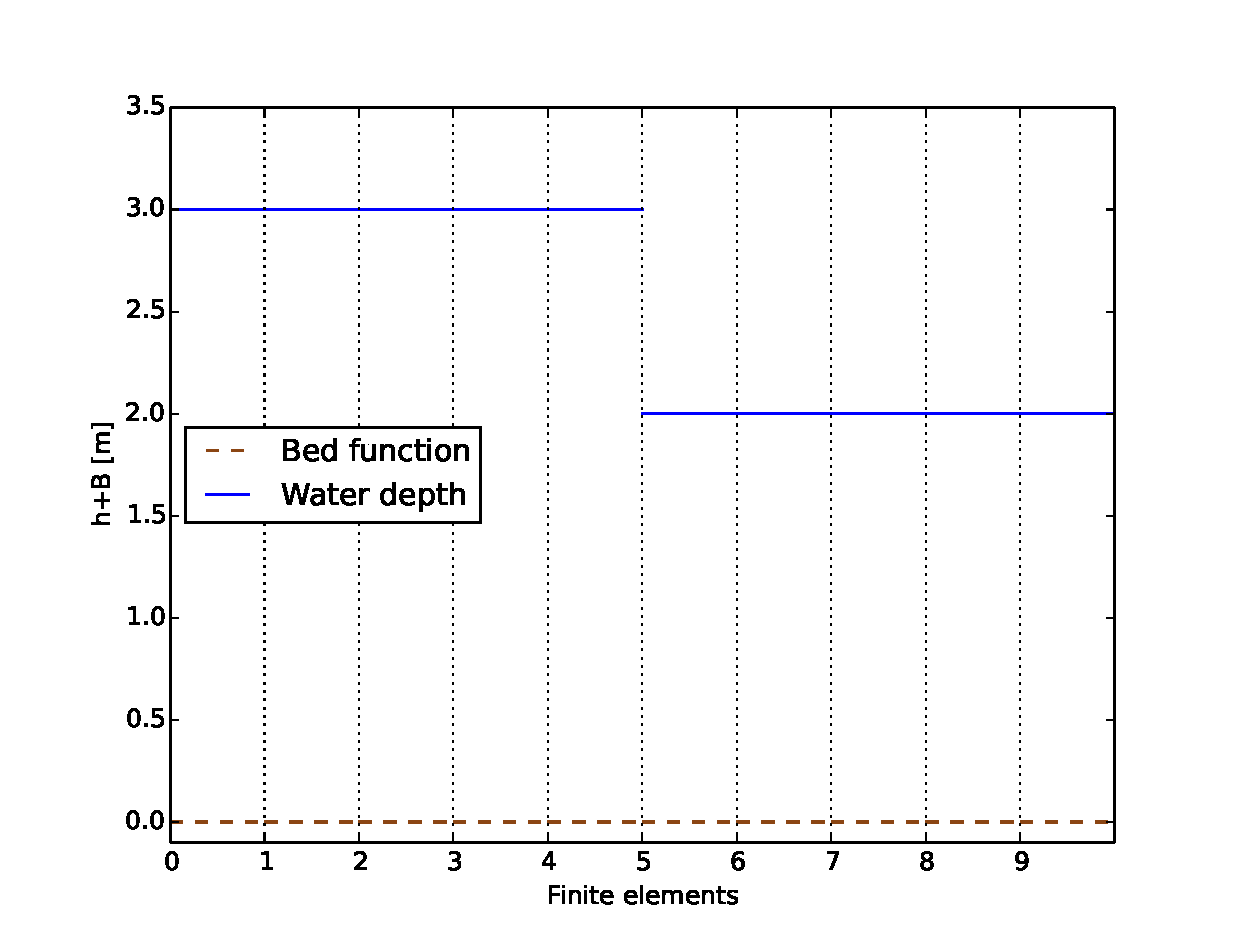
\includegraphics[width=0.7\textwidth]{OBR/riemann.eps}
\caption{Initial conditions of the Riemann problem.}\label{riemann}
\end{figure}
\begin{figure}
\centering
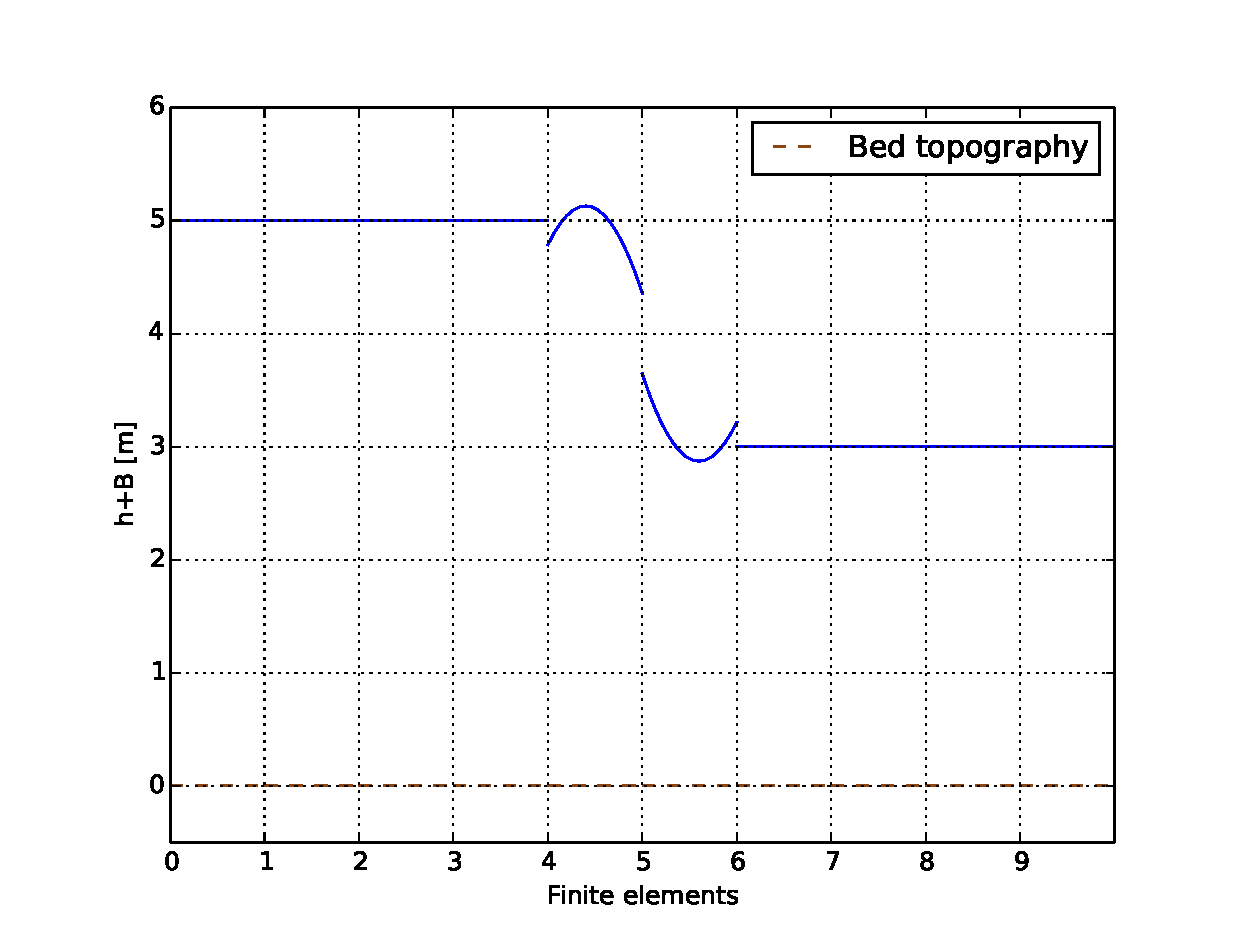
\includegraphics[width=0.7\textwidth]{OBR/first.eps}
\caption{First time iteration of non-limited water depth.}\label{first}
\end{figure}
\begin{figure}
\centering
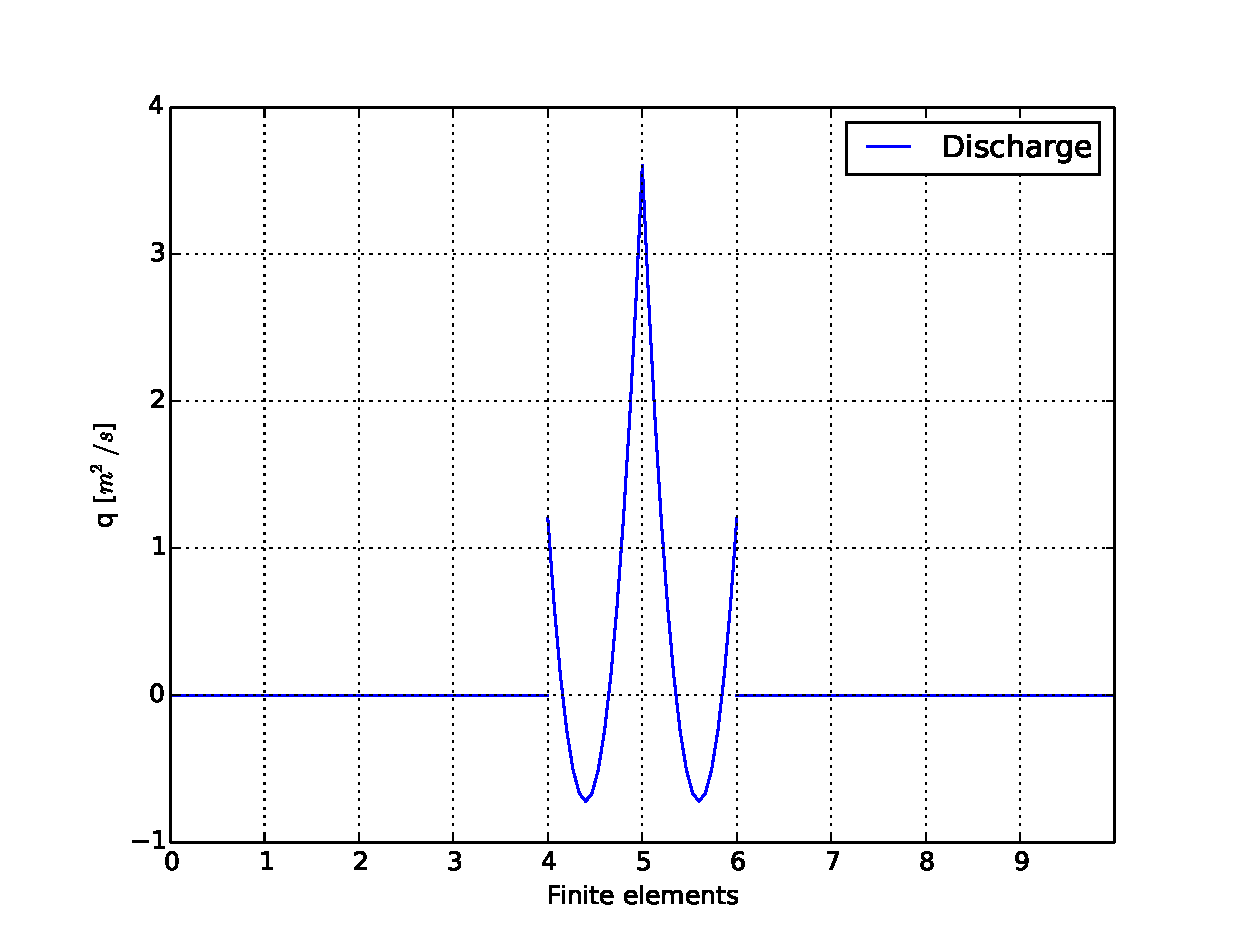
\includegraphics[width=0.7\textwidth]{OBR/HU.eps}
\caption{First time iteration of non-limited discharge.}\label{HU}
\end{figure}
It is very likely that non-limited solution around the shock is not monotone and concave or convex as shown for water depth and discharge in Figures \ref{first} and \ref{HU}. The novel criterion for the second order polynomial base functions suppose, that the solution in the centre of the finite element must be bounded by the values at the edge of this element. If the solution in the middle is not bounded, i.e.
\begin{equation}\label{crit}
\begin{array}{c}
 min\left(W_{i,k}(x_{i-\frac12},t),W_{i,k}(x_{i+\frac12},t\right)>W_{i,k}(x_i,t)\\
\text{or}\\
 max\left(W_{i,k}(x_{i-\frac12},t),W_{i,k}(x_{i+\frac12},t)\right)< W_{i,k}(x_i,t)
 \end{array}
\end{equation}
the cell is defined as 'troubled' and the solution of a conservative variable must be limited in this cell.

The solution in the 'troubled' cells must be limited. The limiting process, used within this work, is similar to the limiting process of Cockburn and Shu \cite{Cockburn1989b}. This process consist in lowering the polynomial order and employing suitable limiter. As a basis functions the Legendre polynomials are used.

 This polynomials can bee seen in Table \ref{table:legendre}.
\begin{table}
\caption{Legendre polynomials}
\centering
\begin{tabular}{|c|c |}
\hline
Base function & Legendre polynomial\\
\hline
\hline
$\varphi^1$ & 1\\
$\varphi^2$ & x\\
$\varphi^3$ & $\frac12\left(3x^2-1\right)$\\
\hline
\end{tabular}
\label{table:legendre}% is used to refer this table in the text
\end{table}
Let us consider the range of these polynomials $[-1,1]$. Interval $[-1,1]$ can be mapped to the arbitrary interval $[x_{i-\frac12},x_{i+\frac12}]$ by linear transformation (linear mapping)
\begin{equation}\label{mapping}
x=x_{i-\frac12}\frac{1-\xi}{2}+x_{i+\frac12}\frac{1+\xi}{2}, \quad x\in[x_{i-\frac12},x_{i+\frac12}],
\quad \xi\in[-1,1].
\end{equation}

  Legendre polynomials are orthogonal in 'integral average' norm, i.e.
\begin{equation}
\int_{-1}^{1} \varphi^j \varphi^l dx \begin{cases}
=0 \text{ for }i\neq j\\
\neq 0 \text{ for }i=j\\
\end{cases}
\end{equation}
thus the integral averages of $\varphi^2$ and $\varphi^3$ are zero\footnote{The integral averages of higher Legendre functions are zero because of the orthogonality with the first one $\int_{-1}^{1} \varphi^{j}\cdot \underbrace{1}\limits_{\varphi^{1}} \ dx=0, \ j=2,3$.} itself and the scheme is still mass and momentum conservative even if the third coefficient $w_{i,k}^{3}$ from (\ref{linC}) is set to be zero.


 Within this work, the minmod limited was chosen to modify the second coefficient
\begin{equation}\label{clasLim}
w_{i,k}^{2}=minmod(\delta^- W_{i,k},\delta^+ W_{i,k})
\end{equation}
where upwind and downwind differences $\delta^\mp W_{i,k}$ are defined by (\ref{diff}) and $minmod$ function is defined as \cite{Nessyahu}
\begin{equation}\label{limiter}
\text{minmod}(z_1,z_2)=\frac{1}{2}[\text{sgn}(z_1) + \text{sgn}(z_2)] \cdot \text{min}(|z_1|, |z_2|).
\end{equation}

\subsection{Implementation of the Surface Gradient Method}
In \cite{Zhou2001}, the Surface Gradient Method (SGM) was introduced. This method has been developed for reconstruction of the water level within the shallow water equations with bed slope source terms. In contrast
to conventional data reconstruction methods based on water depth ($h$) the
water surface level ($h+B$) is chosen as the basis for data reconstruction. This provides
accurate values of the conservative variables at cell interfaces so that the fluxes can
be accurately calculated with a Riemann solver.

If the SGS method is adopted, the 'troubled' cell criterion (\ref{crit}) is defined as
\begin{equation}\label{critH}
\begin{array}{c}
 min\left(W_{i,1}(x_{i-\frac12},t)+B(x_{i-\frac12}),W_{i,1}(x_{i+\frac12},t)+B(x_{i+\frac12})\right)>W_{i,1}(x_i,t)+B(x_i)\\
\text{or}\\
 max\left(W_{i,1}(x_{i-\frac12},t)+B(x_{i-\frac12}),W_{i,1}(x_{i+\frac12},t)+B(x_{i+\frac12})\right)< W_{i,1}(x_i,t)+B(x_i)
 \end{array}
\end{equation}
The limiting process is similar to the process described earlier. The third coefficient $w_{i,1}^{3}$ is set to zero. The difference is in computation of the second coefficient $w_{i,1}^{2}$. Upwind and downwind differences used in the limiter (\ref{limiter}) are computed as
\begin{equation}\label{diffH}
\delta^- W_{i,1}=\frac{\left(W_{i,1}+B_{i}\right) - \left(W_{i-1,1}+B_{i-1} \right)}{\Delta x},\quad \delta^+W_{i,1}=\frac{\left(W_{i+1,1}+B_{i+1}\right) - \left(W_{i,1}+B_{i} \right)}{\Delta x}.
\end{equation}
As in the vector of the conservative variable (\ref{konz}), the water depth (instead of the water level) is stored, the second coefficient must be computed as
\begin{equation}
w_{i,1}^{2}=minmod(\delta^- W_{i,1},\delta^+ W_{i,1})-\delta B_i
\end{equation}
where $\delta B_i$ means the slope of the bed function computed as
\begin{equation}
\delta B_i=\frac{B_{i+\frac12}-B_{i-\frac12}}{\Delta x_i}.
\end{equation}
 Provided that the piece-wise linear bed function is also described by the linear combination of the bed function coefficients $w_{i}^j$ and the first two Legendre polynomials
\begin{equation}
 B_i(x)=w_{b_{i}}^1 \cdot 1+w_{b_{i}}^2 \cdot x,
 \end{equation}
 $\delta B_i$ is identical to the coefficient $w_{i}^2$. Index $b$ implicates that the $w_{b_{i}}$ coefficients belong to the description of the bed function.

\section{Wet/dry Interface}

The numerical solvers can yield spurious negative water depth. This non-physical phenomena can occur mainly during the wetting and drying processes in the computational domain as shown in Figure \ref{wetDry}. This phenomena is well known from the theory of finite volumes \cite{audusse, Audusse2005, cotoJe, Casulli2009, 
Fiser2014, Hou2013, Hou2014, Kesserwani2013, Medeiros2013}. In \cite{kurg2}, Kurganov et al. suggested positivity preserving scheme based on finite volume method. This scheme modifies the slope of linear reconstruction so that there is no negative water depth within the finite volume.

 An exemplary finite volume reconstruction resulting in negative water depth 
at the edge $i-\frac12$ is shown in Figure \ref{negW}. The negative 
water depth $h_{i-\frac12}$ at the edge $i-\frac12$ is set to zero and the water 
depth $h_{i+\frac12}$ is computed in such way that the water depth at cell center 
$h_i$ remains unchanged:
\begin{equation}
\begin{array}{c}
\underbrace{0}_{h_{i-\frac12}}+B_{i-\frac12}+\delta h_i \frac{\Delta x_i}{2}=
h_i+\frac{B_{i+\frac12}+B_{i-\frac12}}{2}\\
\Downarrow\\
\delta h_i=\frac{2h_i+B_{i+\frac12}-B_{i-\frac12}}{\Delta x_i}
\end{array}
\end{equation}
Here $\delta h_i$ is the slope of the water level. Then 
\begin{equation}
h_{i+\frac12}=h_i+\frac{B_{i+\frac12}+B_{i-\frac12}}{2}+
\delta h_i \frac{\Delta x_i}{2}-B_{i+\frac12}=2h_i.
\end{equation}
The corrected reconstruction of the water depth is shown in 
Figure \ref{zeroW}.
\begin{figure}[t]
\centering
\begin{minipage}[t]{0.44\textwidth}
\begin{center}
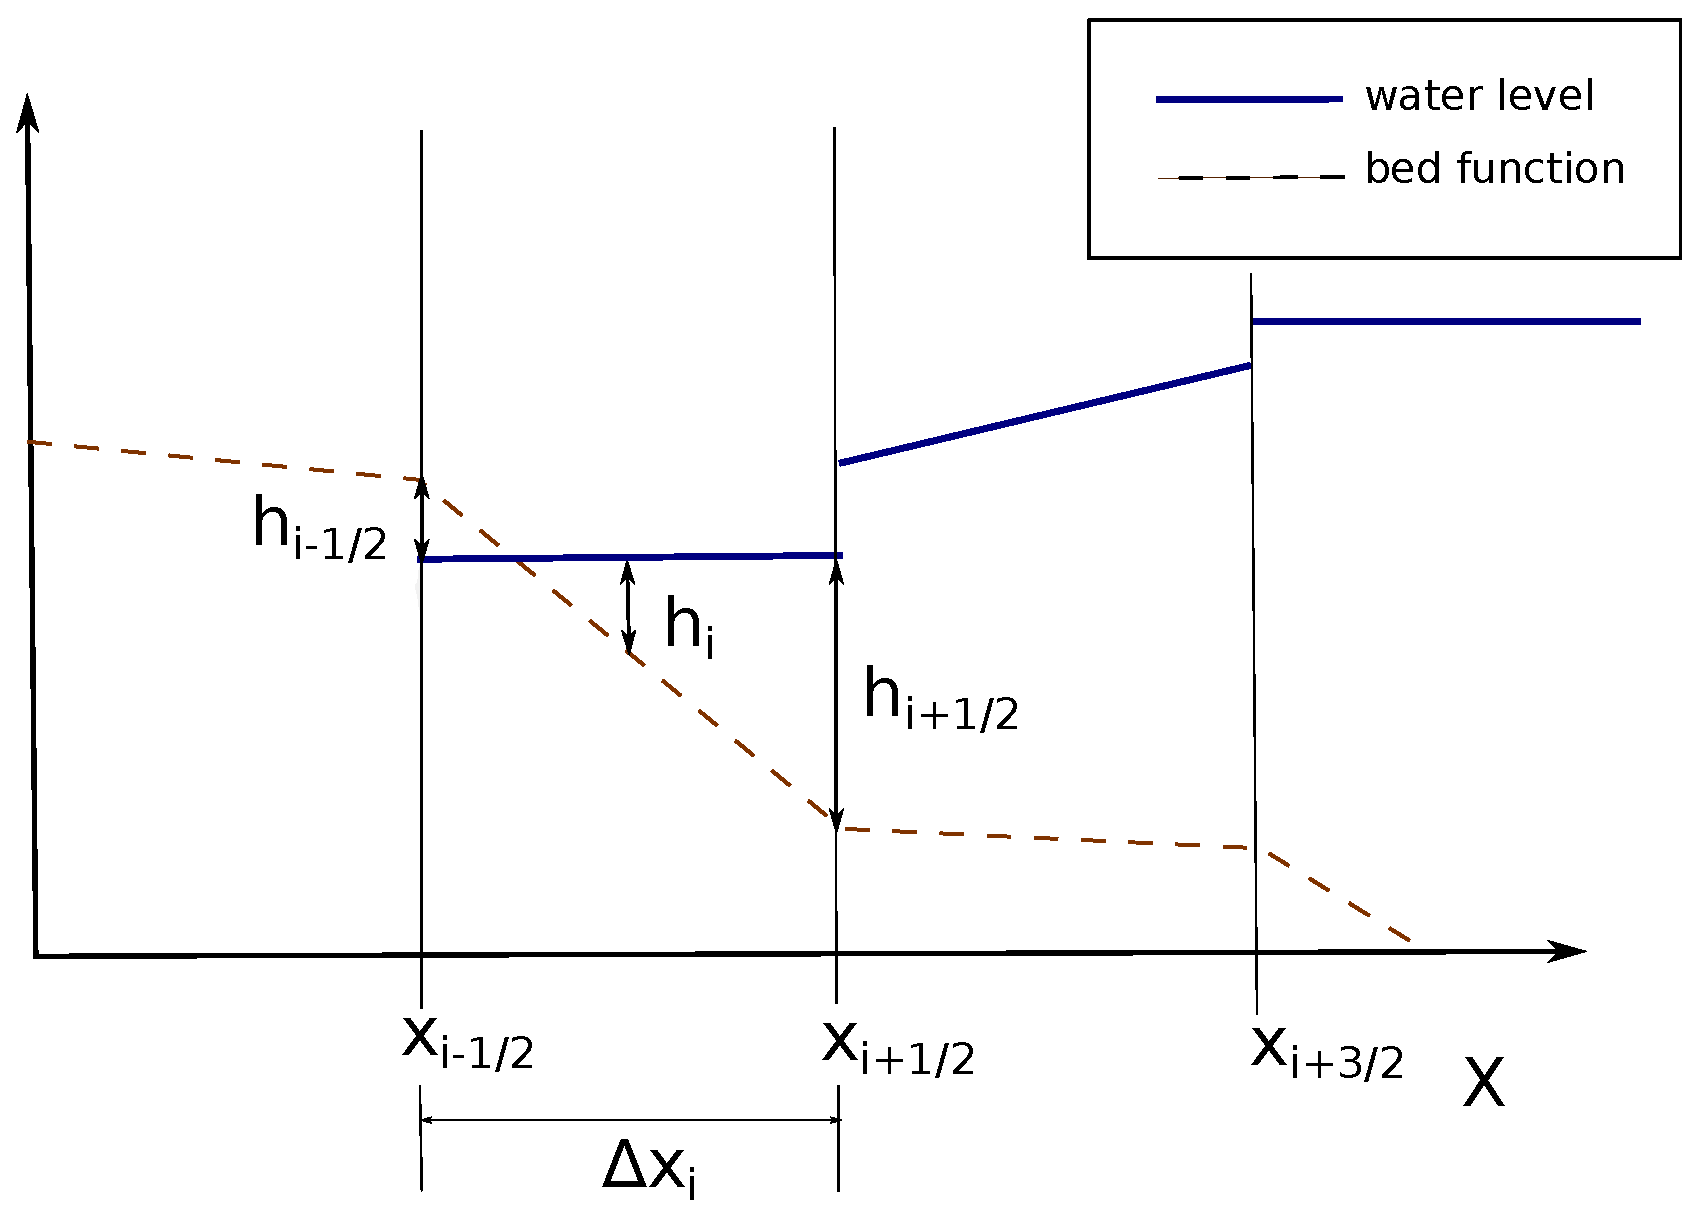
\includegraphics[width=1\textwidth]{OBR/negW.eps}
\caption{Linear reconstruction of the water depth with the negative water depth $h_{i-\frac12}$.}\label{negW}
\end{center}
\end{minipage}\hspace{15mm}
\begin{minipage}[t]{0.44\textwidth}
\begin{center}
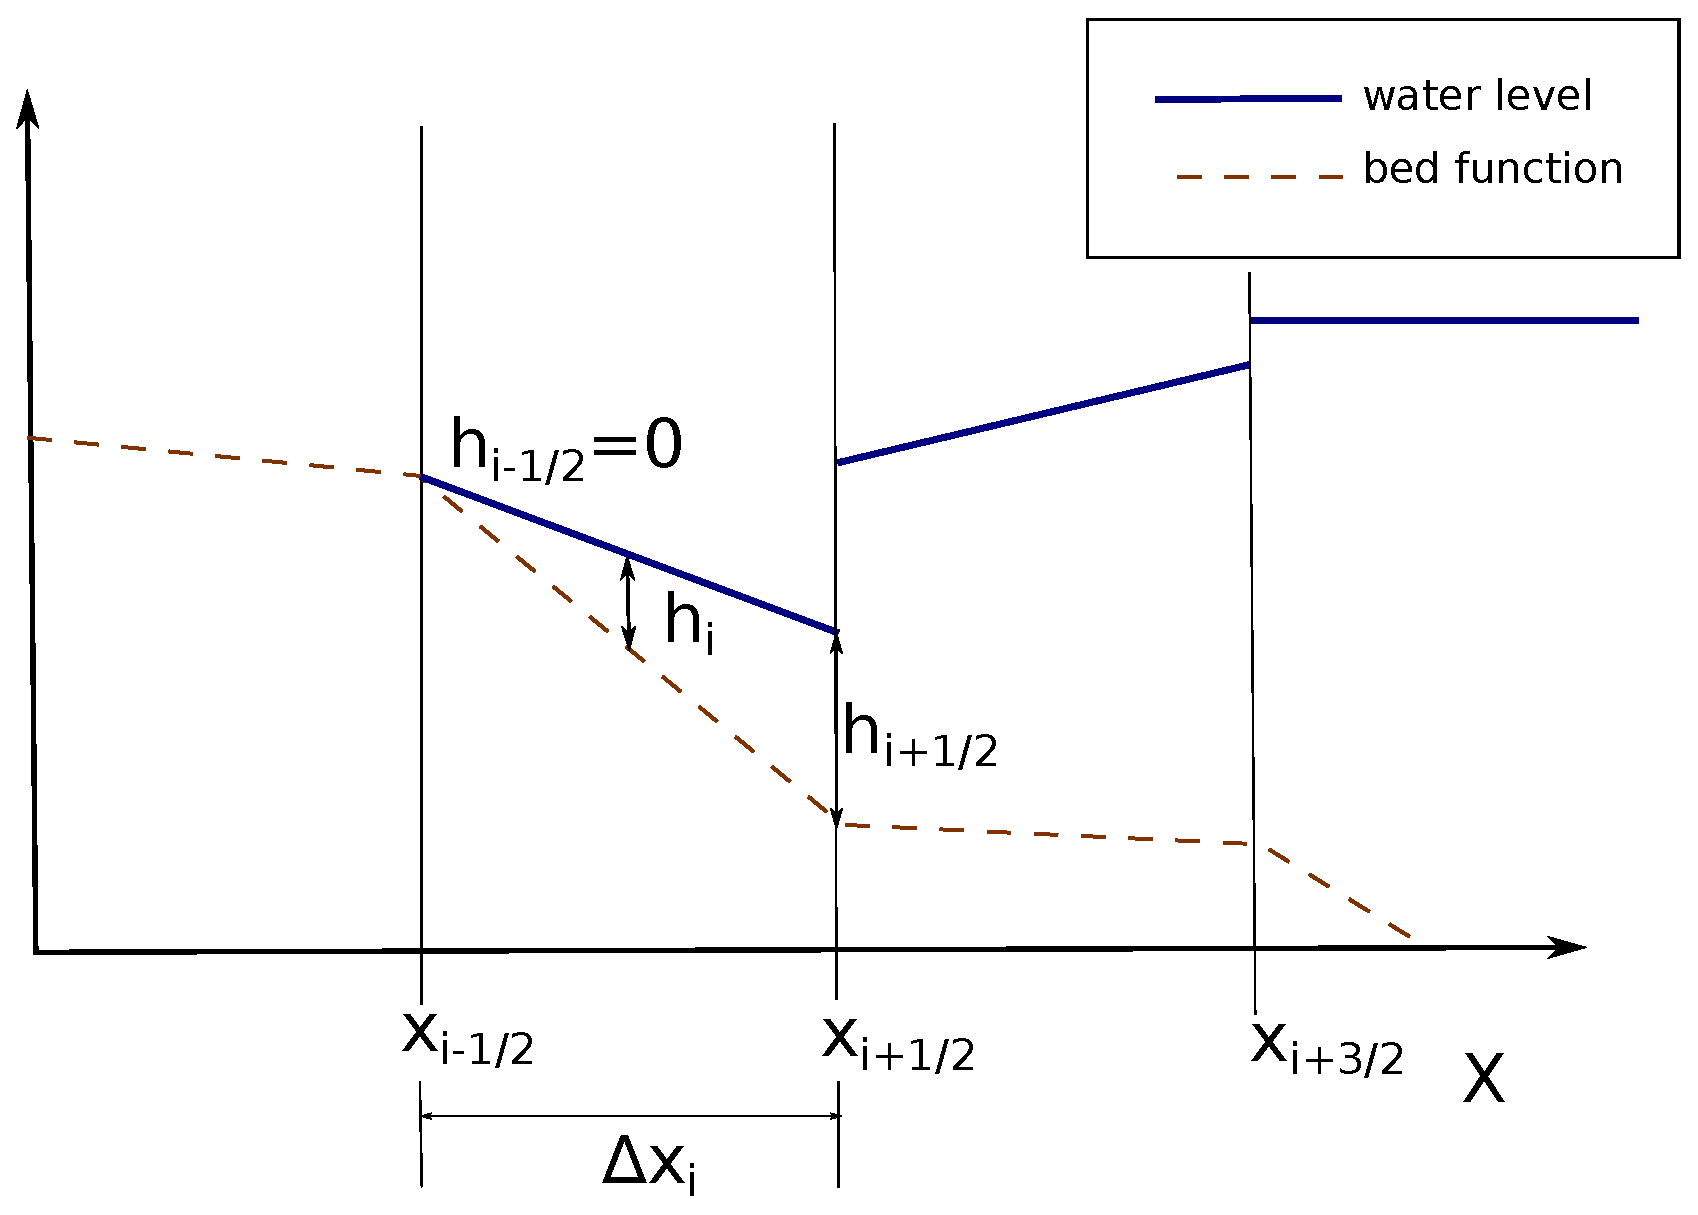
\includegraphics[width=1\textwidth]{OBR/zeroW}
\caption{Corrected linear reconstruction of the water depth.}\label{zeroW}
\end{center}
\end{minipage}
\end{figure}	
The case when $h_{i+\frac12}<0$ can be corrected in a similar way and the conditions of the 
correction can be summarized as \cite{kurg2}
\begin{equation}\label{kurgMod}
\begin{array}{c}
\text{if} \quad h_{i-\frac12}<0 \begin{cases}
h_{i-\frac12}=0\\
h_{i+\frac12}=2h_i
\end{cases},\\
\\
\text{if} \quad h_{i+\frac12}<0 \begin{cases}
h_{i-\frac12}=2h_i\\
h_{i+\frac12}=0
\end{cases}.\\
\end{array}  
\end{equation}
After this modification, the non-negativity of the water depth is ensured. 

Higher order DGFEM method can produce the negative values of the water depth not only at the edges but also within the finite element as shown in Figure \ref{wetDry}.
\begin{figure}
\centering
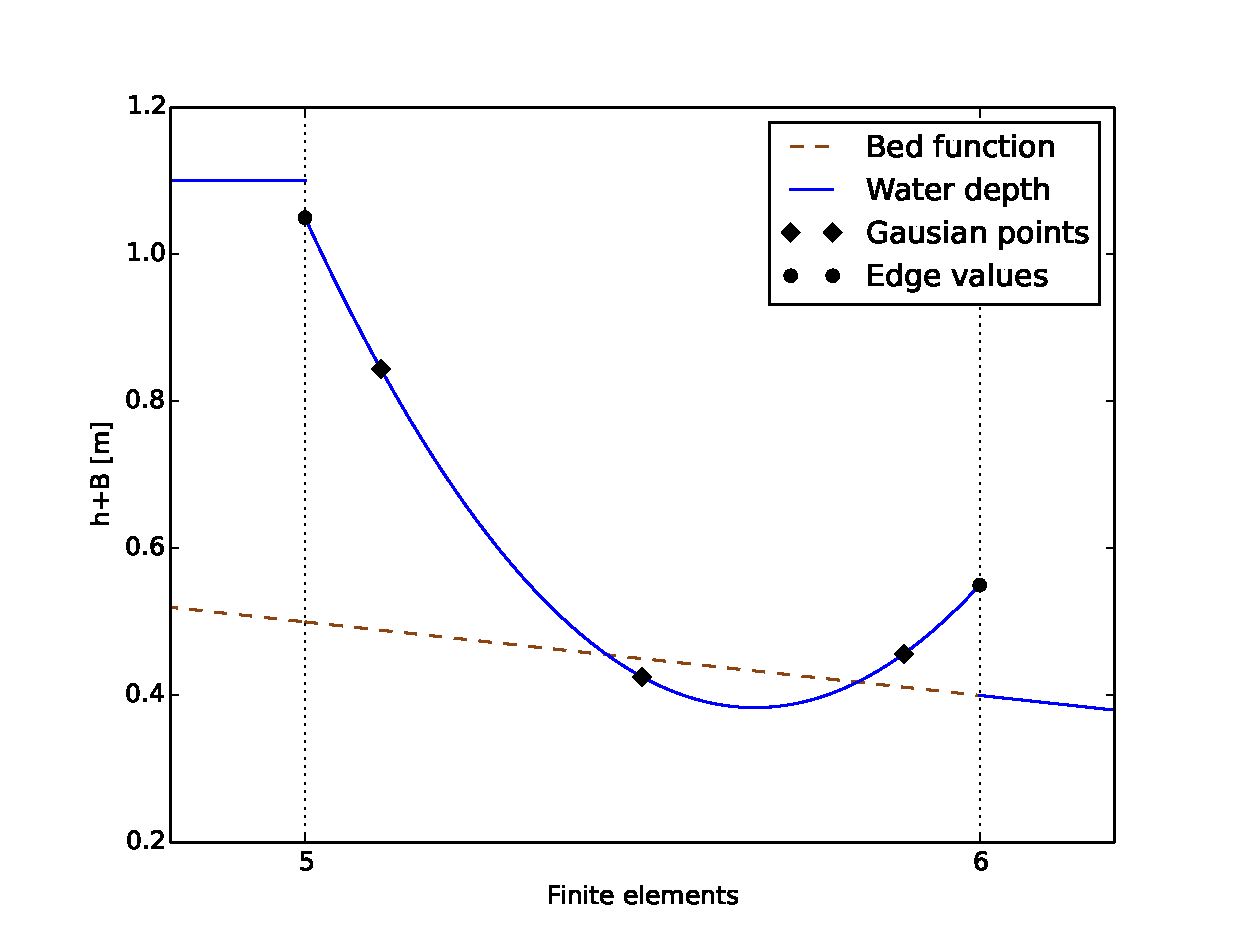
\includegraphics[width=0.7\textwidth]{OBR/wetDry.eps}
\caption{Non-physical solution with negative water depth.}\label{wetDry}
\end{figure}
 It is computationally demanding to check whole solution within the finite element thus we suggest to check the positivity of the solution only in the points which are used for the computations. These points are the Gaussian points and values at the edges of the finite element. This process results in novel criterion for wet/dry interface. The solution must be limited if 
 \begin{equation}
 W_{i,1}(x_p)<0
 \end{equation}
where $x_p$ stands for Gaussian points and points at the edges of the finite element. First part of the limitation of the water depth is similar to that one described in Section \ref{limSec}. The third coefficient is set to be zero which yields the situation depicted in Figure \ref{lin}. 
\begin{figure}
\centering
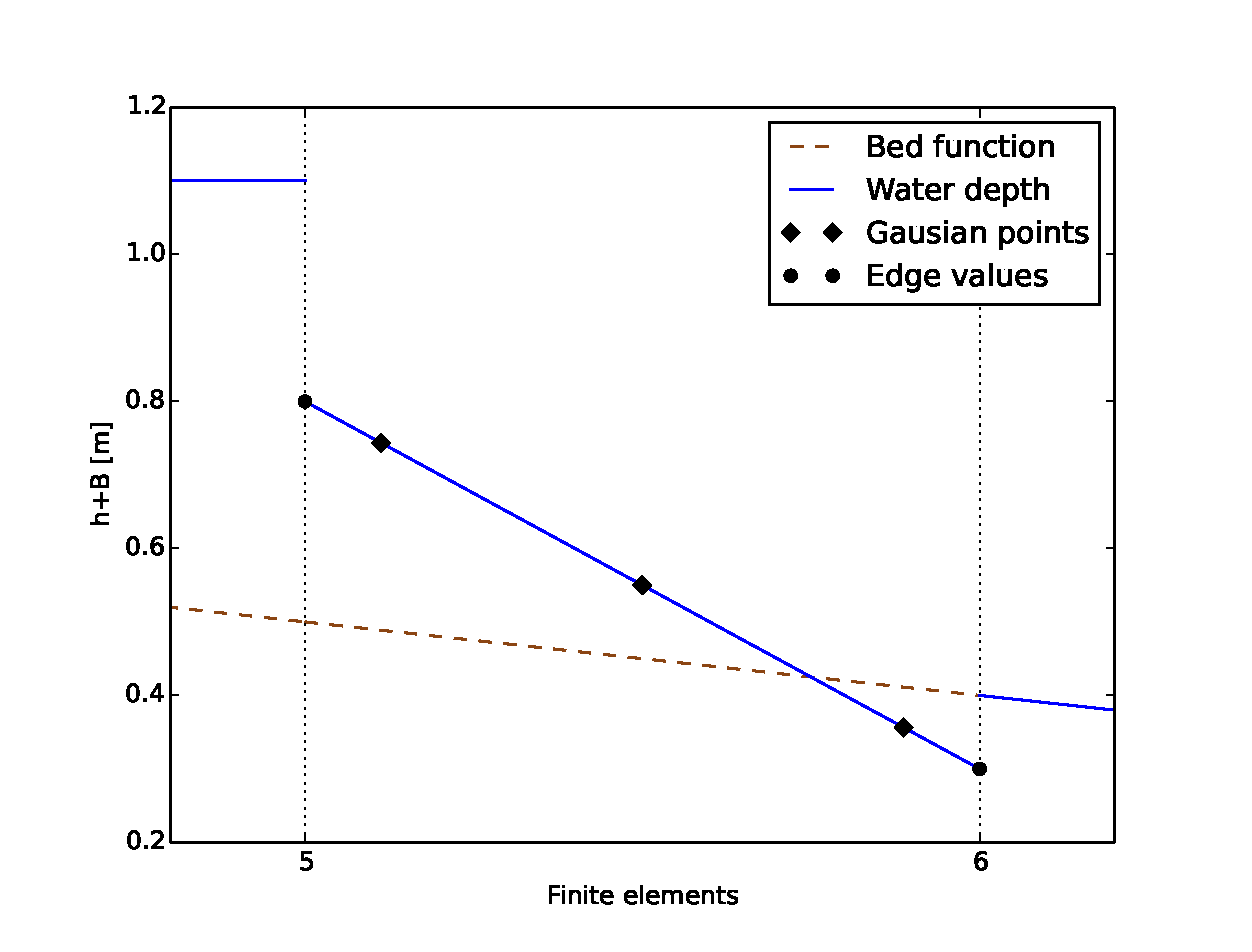
\includegraphics[width=0.7\textwidth]{OBR/lin.eps}
\caption{Limited solution of the water depth.}\label{lin}
\end{figure}
After that, the coefficient $w_{i,1}^2$, governing the slope of the linear function, is altered to gain the same values as in (\ref{kurgMod}). It means that, in case when the water depth $W_{i,1}(x_{i-\frac12})$ is negative, the slope of the function can be computed as
\begin{equation}\label{slope}
w_{i,1}^2=\frac{W_{i,1}(x_{i})-0}{ \frac{\Delta x_i}2}=W_{i,1}(x_{i}).
\end{equation}
Let us highlight that $\Delta x_i=2$ because of the mapping (\ref{mapping}) and after the limitation to the linear function, the value of the water depth in the middle of the finite element is equal to the first coefficient, i.e.
\begin{equation}\label{coefVal}
W_{i,1}(x_{i})=w_{i,1}^1.
\end{equation}
 Taking in account (\ref{coefVal}), relation (\ref{slope}) can be generalised for both edges as
\begin{equation}
w_{i,1}^2=\begin{cases}
w_{i,1}^1, \text{  if  } W_{i,1}(x_{i-\frac12})<0 \\
-w_{i,1}^1, \text{  if  } W_{i,1}(x_{i+\frac12})<0
\end{cases}.\\
\end{equation}
Final limited and corrected solution can be seen in Figure \ref{linCor}.
\begin{figure}
\centering
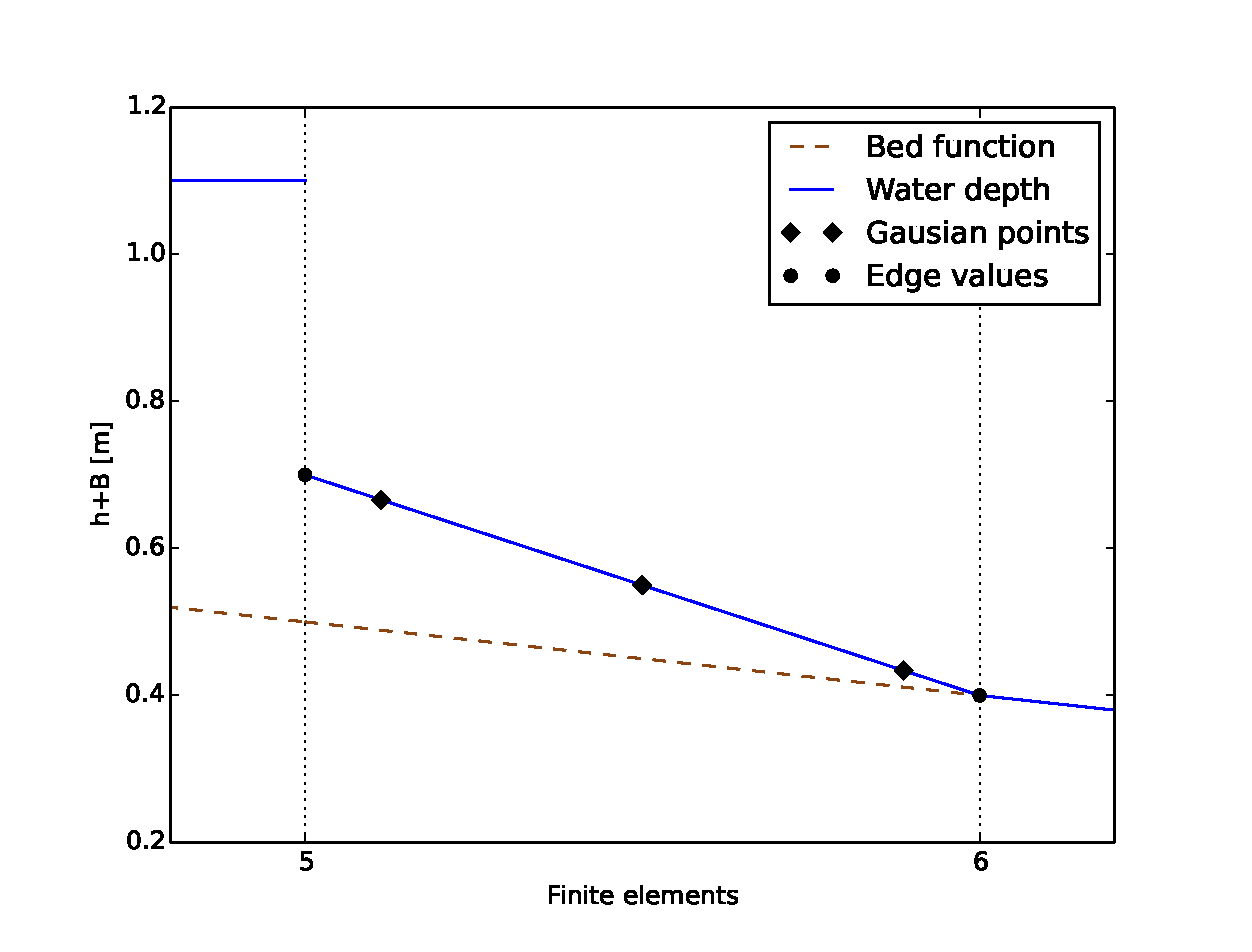
\includegraphics[width=0.7\textwidth]{OBR/linCor.eps}
\caption{Corrected solution of the water depth.}\label{linCor}
\end{figure}




However this water depth may become very small and cause problems with the computation of 
the velocity $u$ which is computed by the fraction of the discharge ($hu$) and water depth $h$ 
\begin{equation}
u=\frac{(hu)}{h}. 
\end{equation}
Obviously $u\rightarrow\infty$ for $h\rightarrow 0$. To avoid unrealistic velocities, 
Kurganov and Petrova \cite{kurg2} proposed the following formulae which 
avoids the division by very small numbers
\begin{equation}\label{formVel}
u=\frac{\sqrt{2}h(hu)}{\sqrt{h^4+\max(h,\epsilon_h)}}.
\end{equation}
$\epsilon_h$ is a small positive constant. In \cite{kurg2} it is 
recommended to set this constant to $\epsilon_h=(\Delta x_i)^4$.
The discharge $hu$, used in the Riemann solver, has to be recomputed as
\begin{equation}
hu=h\cdot u.
\end{equation}


%\section{Bed Friction Source Term}\label{friction}
The bed friction source term is in the mathematical model represented by the bed friction vector (\ref{Sf}), i.e.
\begin{equation}\nonumber
\mathbf{S}_{f}=\begin{bmatrix}                                                  
0 \\                                                                            
-\tau_f\\                                                    
\end{bmatrix},
\end{equation}
with 
\begin{equation}
\tau_f = C_f u |u|
\end{equation}
where $C_f$ stands for 
\begin{equation}\label{CFko}
C_f=g \frac{n^2}{\sqrt[3]{h}}
\end{equation}
and $n$ is Manning's bed roughness factor.

Because of the bed friction the time integration of the Equation \ref{semi} must be done in two steps. First, the semi-discrete scheme without the bed friction term
\begin{equation}\label{semiB2}
\frac{\text{d}}{\text{d}t}\mathbf{w}_{i,k}= \mathbf{M}_i^{-1}\mathbf{RHS}_{i,k}
\end{equation}
is integrated. Equation \ref{semiB2} yields the solution $\mathbf{w}^{n+\frac12}_{i,k}$ where upper index $n+\frac12$ means the time level. When wetting and drying processes appear in the numerical simulation, the bed friction source term dominates the stability of the numerical scheme due to the water depth in the denominator of (\ref{CFko}). Thus the special limiter must be implemented.

 Within this work we suggest the limiter which is similar to the finite volume limiter described in \cite{marche}. The bed friction affects only momentum equation, thus the limiter must be used only for $k=2$ and we define this limiter as
  \begin{equation}\label{fricCase}
\mathbf{w}_{i,2}^{n+1}=
\begin{cases}
                \mathbf{w}_{i,2}^{*}   \quad  \quad  \text{if} \quad sign\left(W_{i,2}\left(\mathbf{w}^{n}_{i,2}\right)\right)=
sign\left(W_{i,2}\left(\mathbf{w}_{i,2}^{*}\right)\right) ,\\
                \mathbf{0} \quad \text{otherwise,}
\end{cases}
\end{equation}
where
\begin{equation}
\mathbf{w}_{i,2}^{*}=\mathbf{w}_{i,2}^{n+\frac12}+\Delta t \mathbf{M}_i^{-1}
 \prescript{f}{}{\mathbf{RHS}}_{i,2}
\end{equation}
and $\mathbf{0}$ is the zero vector. Equation \ref{fricCase} de facto means that the discharge $W_{i,2}=(hu)_i$ is set to be zero in the case when the bed friction term changes the flow direction.


\section{Numerical Results}
In this section, the novel scheme is validated against analytical solutions and compared with other schemes.

\subsection{Dam Break on a Wet Domain without Friction}\label{DBwet}
This benchmark is a classical Riemann problem which can be represented by a dam separating two basins with different water depths. The dam is instantaneously removed and the flow patterns are simulated. The analytical solution was firstly introduced in \cite{stoker}. Simple overview of this solution can be also found in \cite{swashe}. The initial conditions of the water depth within our simulation are 
\begin{equation}
h(x)=\begin{cases}
h_l, \text{ for } 0<x<x_0\\
h_r, \text{ for } x_0<x<L\\
\end{cases}
\end{equation}
where $h_l=5$ m, $h_r=3$ m, the position of the dam is $x_0=5$ m and the length of the computational domain is $L=10$ m. The computation is stopped at the time $t=0.5$ s and compared with the DGFEM global limiting scheme (DGFEM GL) where the minmod limiter was used for the shock detection. The solution of the water level can be seen in Figure \ref{shock}. This figure shows the results computed by ten finite elements. 
\begin{figure}
\centering
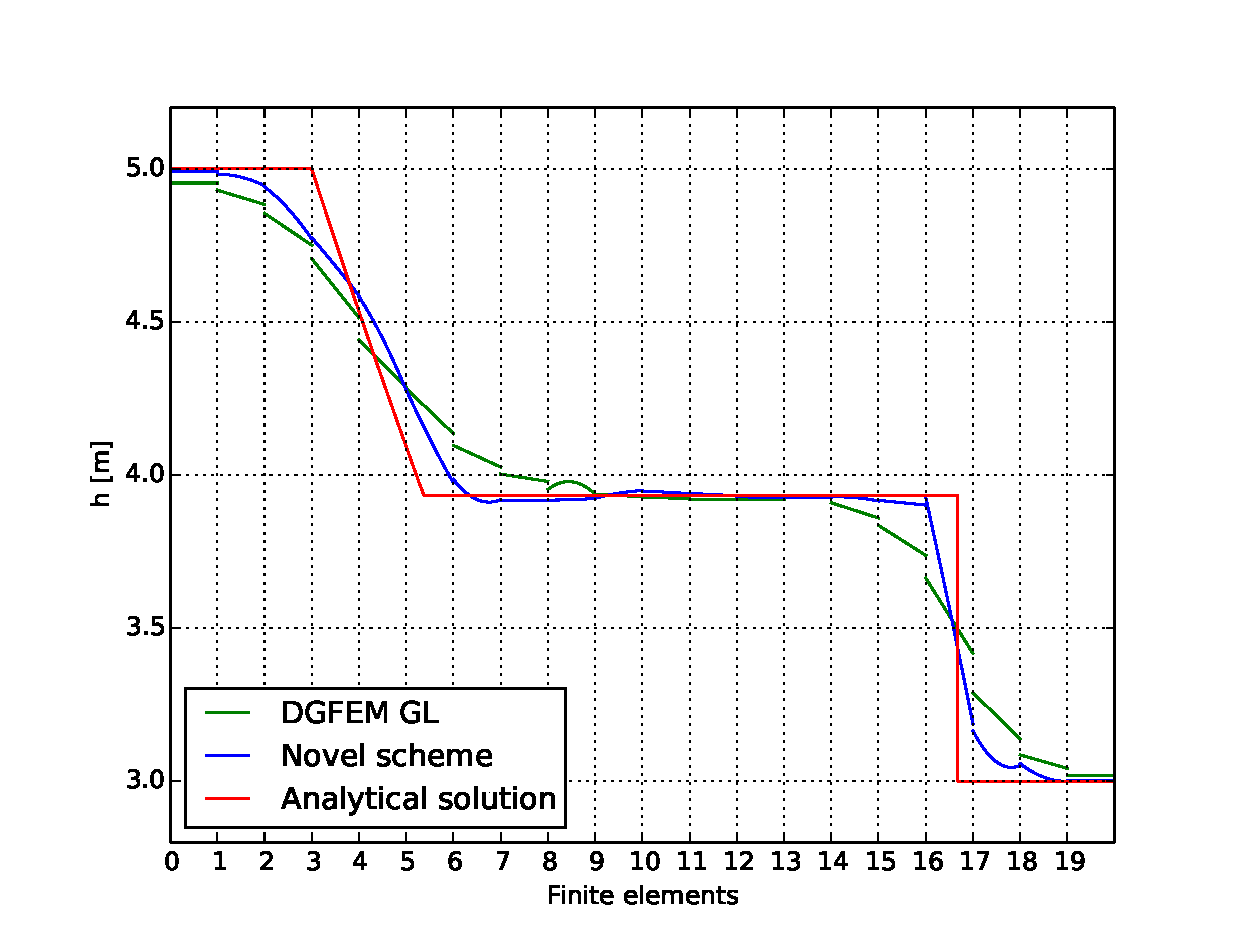
\includegraphics[width=0.7\textwidth]{OBR/shock.eps}
\caption{Simulation of the water level. Comparison of the global limiting and novel scheme.}\label{shock}
\end{figure}
The convergence of a scheme for given test case can be found by the slope of the $log(L_2 \text{error})$ dependent on $log(n_t)$. This slope can bee seen in Figure \ref{L2}. $L_2$ error was computed as
\begin{equation}\label{L2er}
L_2 \text{ error}=\sqrt{\frac{\sum_{i=1}^{n_t} (h_n(x_i)-h_a(x_i))^2 \Delta x_i}{L} }
\end{equation}
where $x_i$ are middle points of the finite elements, $\Delta x_i$ is cell width and $h_{n}$/$h_a$  means the numerical/analytical solution. The slopes of the convergence in Figure \ref{L2} were computed by the linear regression of $L_2$ errors. Numerical results shown that the novel scheme gives better accuracy and convergence of the DGFEM.
\begin{figure}
\centering
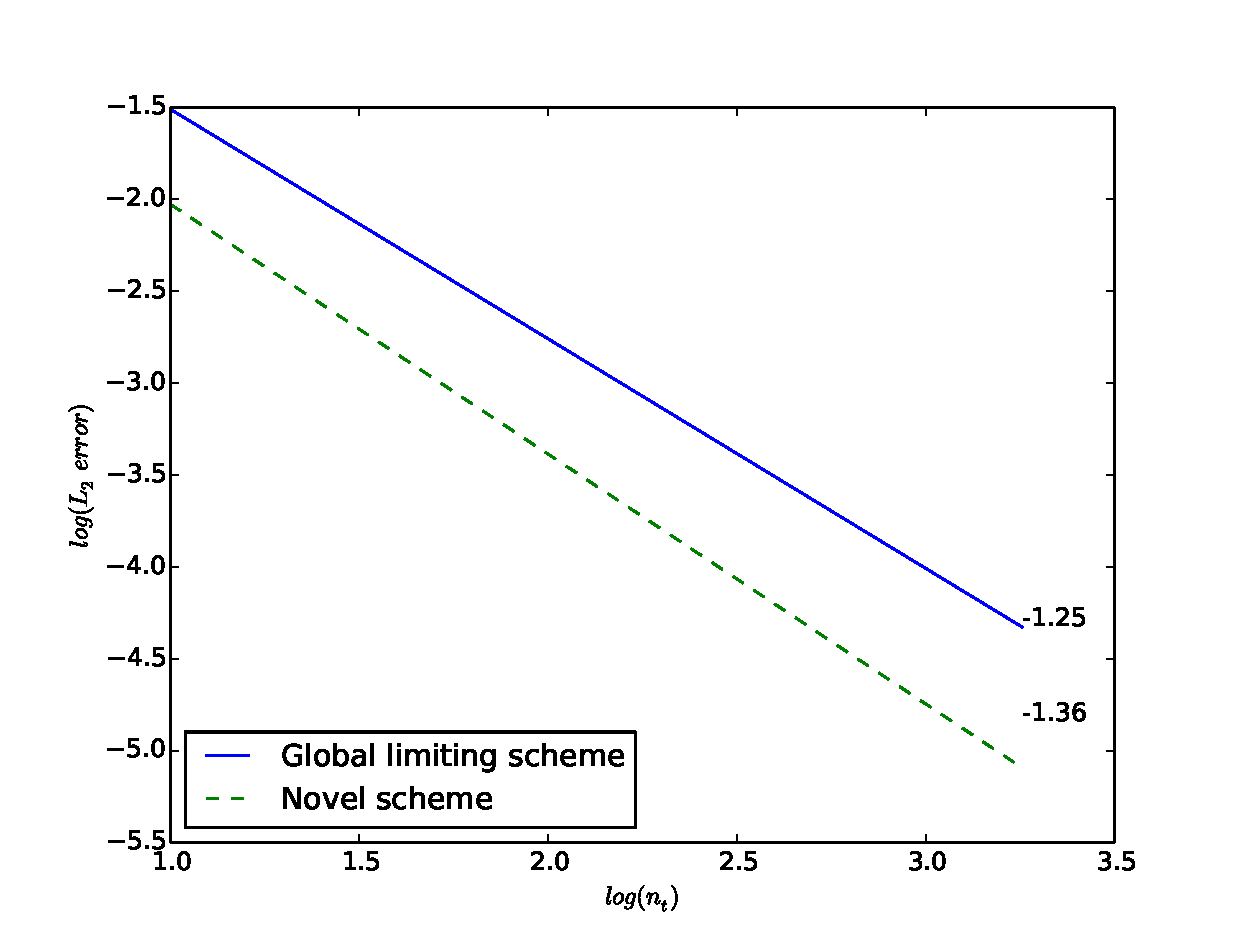
\includegraphics[width=0.7\textwidth]{OBR/shockConverg.eps}
\caption{$L_2$ error convergence of the global limiting and novel scheme.}\label{L2}
\end{figure}


\subsection{Planar surface flow in a parabola}\label{psp}
Another benchmark is the planar surface in a parabola without friction. In this bench mark the the wetting and drying processes occur. Two-dimensional exact solution was derived in \cite{Thacker2006}. 
Here, one-dimensional simplification presented in \cite{swashe} is computed. 
The topography is a parabolic shape given by 
\begin{equation}
B(x)=h_0 \left( \frac{1}{a^2}\left(x-\frac{\text{L}}{2}
\right)^2-1\right).
\end{equation}
The analytical solution of the water depth is
\begin{equation}\label{initPar}
h(x)=\begin{cases}
-h_0 \left(\left(\frac{1}{a}\left(x-\frac{\text{L}}{2}\right)
+\frac{C}{\sqrt{2gh_0}}\cos\left(\frac{\sqrt{2gh_0}}
{a}t\right)\right)^2-1\right) \quad \text{for} 
\ x_1(t)\leq x\leq x_2(t),\\
0 \quad \text{otherwise},
\end{cases}
\end{equation}
with location of the wet/dry interfaces at time $t$ being calculated as
\begin{equation}
\begin{array}{c}
x_1(t)=-\frac12\cos\left(\frac{\sqrt{2gh_0}}{a}t\right)
-a+\frac{\text{L}}{2},\\
x_2(t)=-\frac12\cos\left(\frac{\sqrt{2gh_0}}{a}t\right)
+a+\frac{\text{L}}{2}
\end{array}
\end{equation}
and 
\begin{equation}
C=\sqrt{\frac{2gh_0}{2a}}.
\end{equation}
Initial conditions of the water depth are given by (\ref{initPar}) for $t=0$~s and the flow velocity is zero.

 In the simulation the following parameters were used: $a=1$ m, $h_0=0.5$ m and $L=4$ m. Comparison of the simulations and analytical solution was done in time  $T=5\frac{a\pi}{\sqrt{2gh_0}}$. For the comparison $L_2$ error (\ref{L2er}) was used. Novel scheme is compared by the second order accurate DGFEM scheme. Within second order accurate scheme, the solution is described by the linear function, thus minmod limiter and global limiting method was used for the limiting of the solution. Moreover the scheme was compared with the finite volume scheme with linear reconstruction presented in \cite{fiser2016}. Visual comparison with the exact solution, for different numbers of finite elements/volumes, can be seen in Figures \ref{10}, \ref{20}, \ref{30} and \ref{40}. 
				\begin{figure}[!ht]
								\centering
								 \begin{minipage}[t]{0.44\textwidth}
								    \begin{center}
								    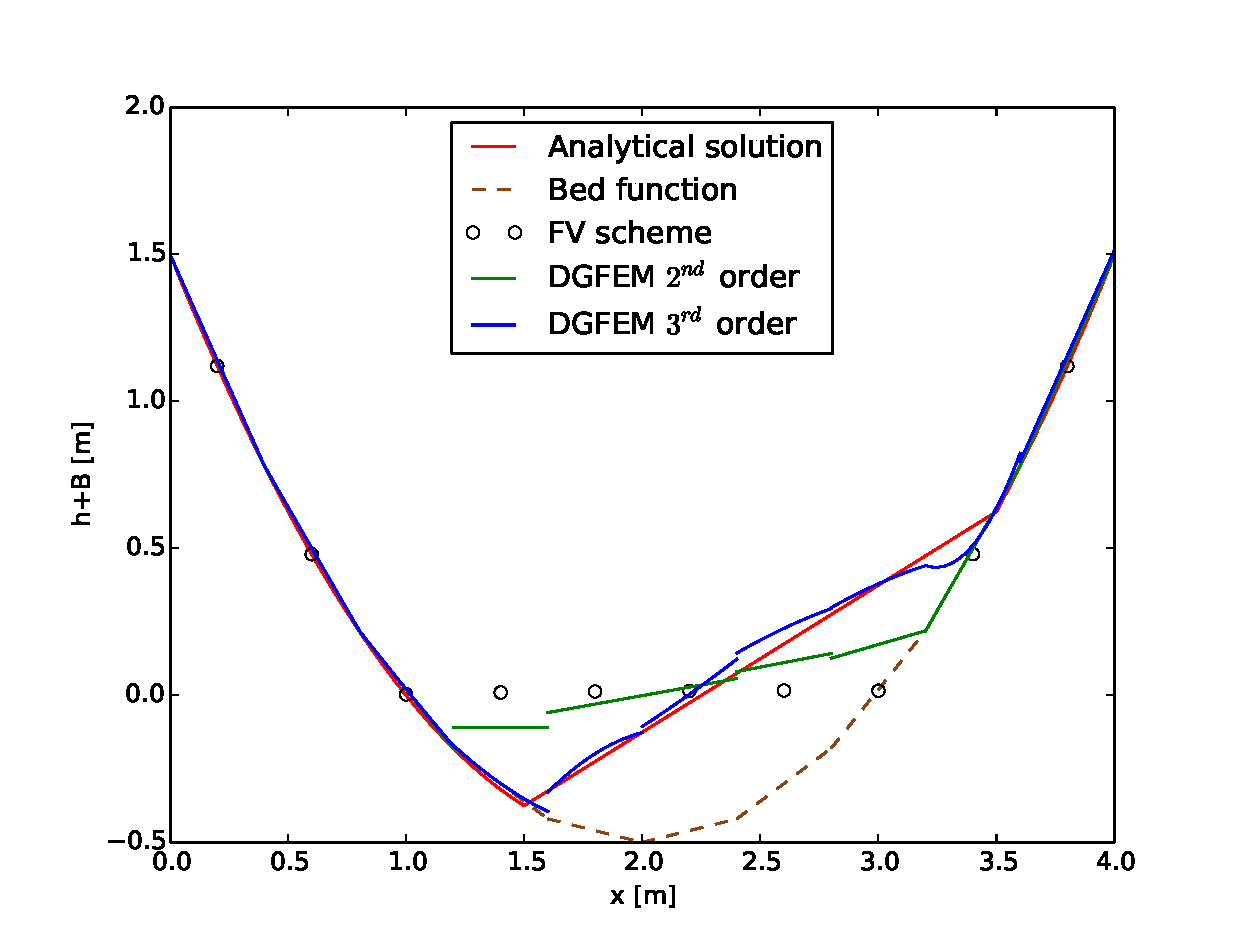
\includegraphics[width=1.0\textwidth]{OBR/10.eps}
								    \caption{Analytical solution compared with the novel and reference scheme-10 finite elements/volumes.}\label{10}
								    \end{center}
								\end{minipage}\hspace{15mm}
								\begin{minipage}[t]{0.44\textwidth}
								    \begin{center}
								    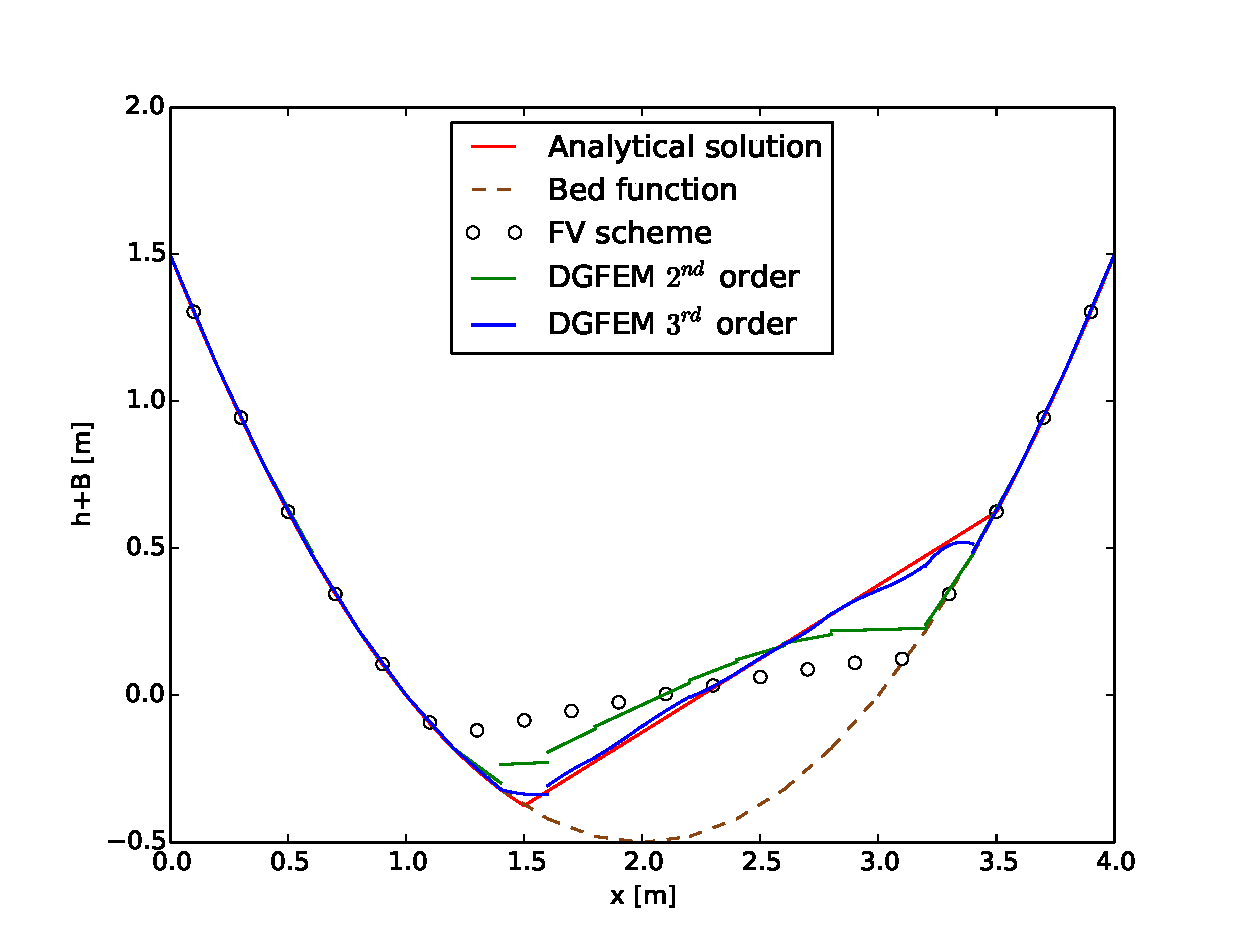
\includegraphics[width=1.0\textwidth]{OBR/20.eps}
								    \caption{Analytical solution compared with the novel and reference scheme-20 finite elements/volumes.}\label{20}
								    \end{center}
								\end{minipage}
				\end{figure}
\begin{figure}[!ht]
								\centering
								 \begin{minipage}[t]{0.44\textwidth}
								    \begin{center}
								    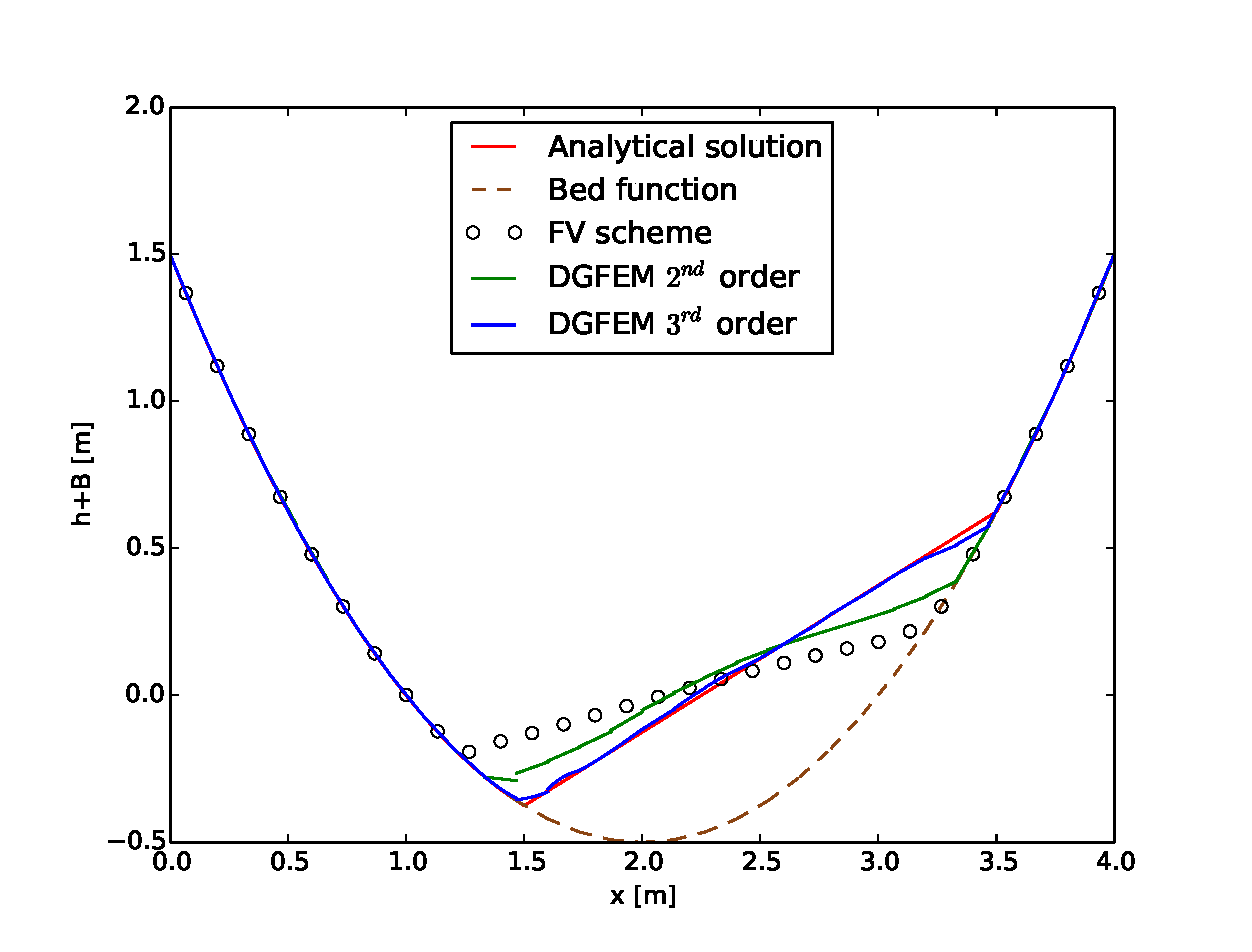
\includegraphics[width=1.0\textwidth]{OBR/30.eps}
								    \caption{Analytical solution compared with the novel and reference scheme-30 finite elements/volumes.}\label{30}
								    \end{center}
								\end{minipage}\hspace{15mm}
								\begin{minipage}[t]{0.44\textwidth}
								    \begin{center}
								    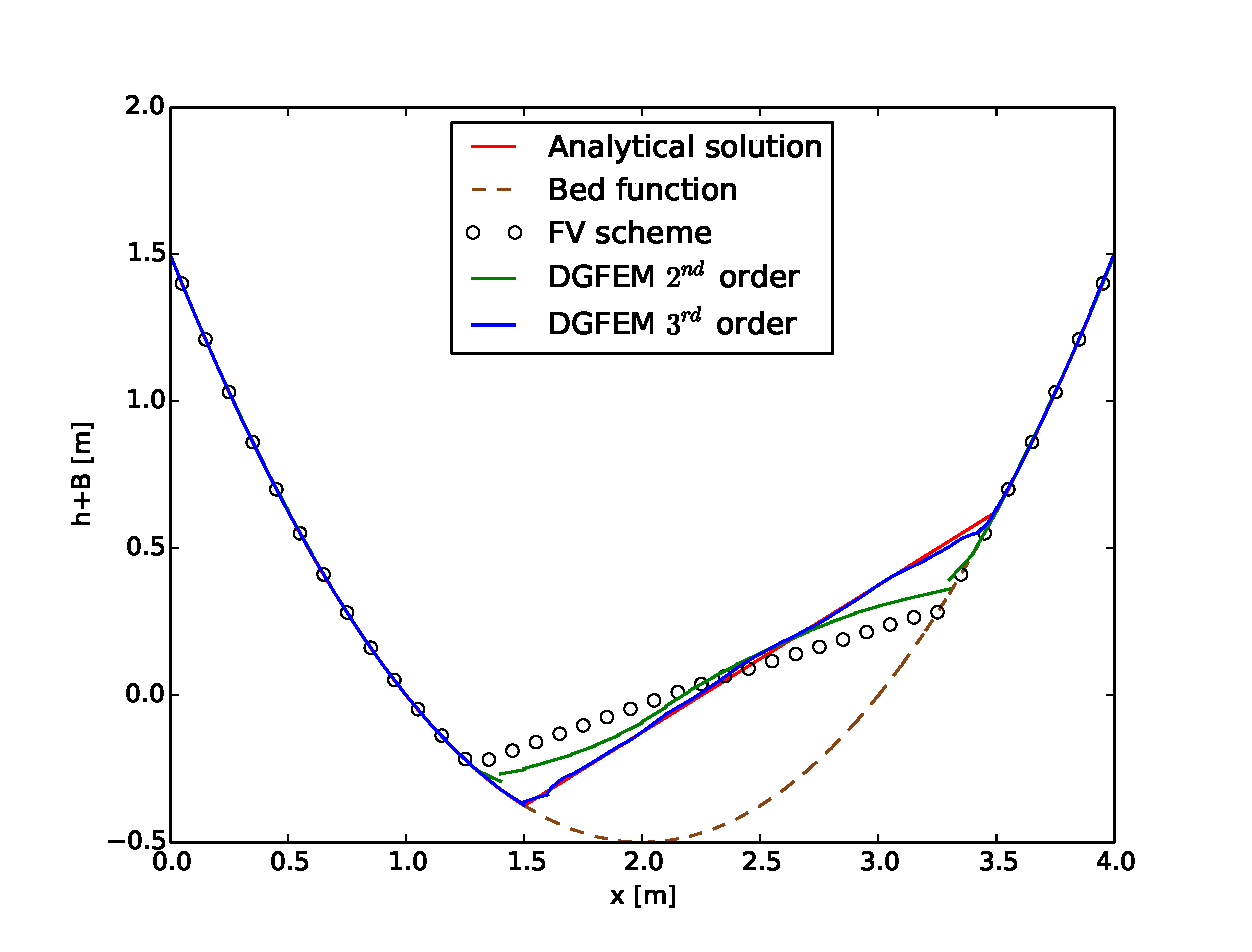
\includegraphics[width=1.0\textwidth]{OBR/40.eps}
								    \caption{Analytical solution compared with the novel and reference scheme-40 finite elements/volumes.}\label{40}
								    \end{center}
								\end{minipage}
				\end{figure}
$L_2$ error convergence is shown in Figure \ref{ParL2}.
\begin{figure}
\centering
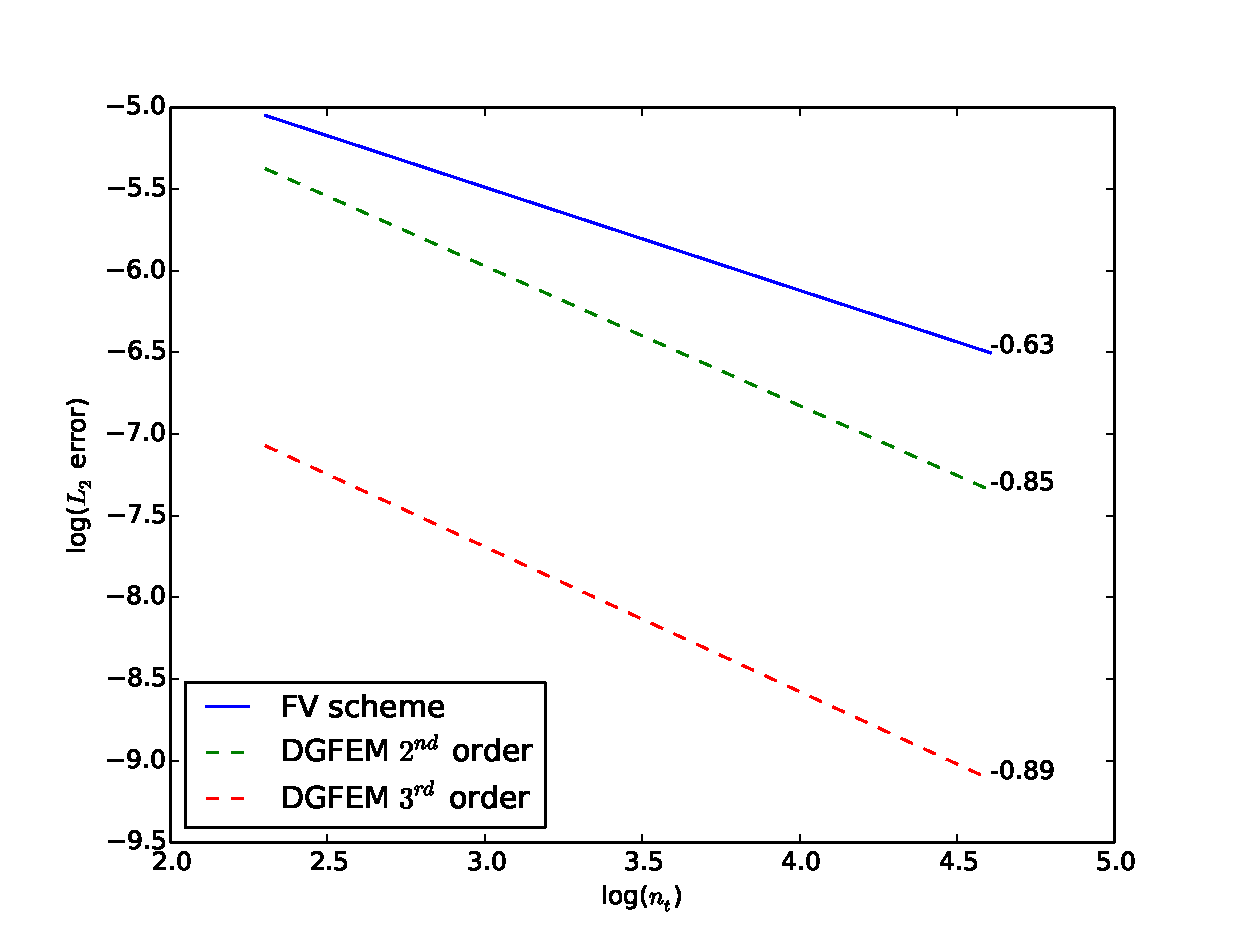
\includegraphics[width=0.7\textwidth]{OBR/ParL2.eps}
\caption{$L_2$ error convergence of the reference FV scheme and novel DGFEM scheme.}\label{ParL2}
\end{figure}

\subsection{Flow over the Bump}
 Another testing benchmark is steady state flow over the bump. The length of the computational domain is L=25 m with a topography given by
\begin{equation}
B(x)=\begin{cases}
 0.2-0.05(x-10)^2  & \text{if 8 m} < x < \text{12 m},\\
0  & \text{else.}
\end{cases}
\end{equation}
In the following, the numerical results of subcritical flow, transcritical flow and transcritical flow with the shock are shown. The results were computed for coarse mesh created by 20 finite elements. The inlet is set on the left side of the computational domain and the outlet is set on the right side of the computational domain. Initial conditions for all these three types of flow are 
\begin{equation}
\begin{array}{ccc}
h(x)+B(x)=2,  \  x\in \Omega,\\
u(x)=0, \ \ \  \qquad \  \  x\in \Omega.
\end{array}
\end{equation}
Analytical solutions of steady state flows over the bump can be found for example in \cite{swashe} or \cite{henderson}. Novel limiting method was also compared with the global limiting method where the minmod limiter was used for the location of the shock.
 
 The boundary conditions of the subcritical flow are
\begin{equation}
\begin{array}{c}
q_{inlet}=4.42 \ m^2/s\\
h_{outlet}=2 \ m
\end{array}
\end{equation}
and the water depth is given by the resolution of 
\begin{equation}
h^3(x)+\left( B(x)-\frac{q _{inlet}^2}{2g h_{outlet}^2}-h _{outlet}\right)h^2(x)+\frac{q _{inlet}}{2 g}=0,\quad \forall x \in [0,L]
\end{equation}

				\begin{figure}[!ht]
								\centering
								 \begin{minipage}[t]{0.44\textwidth}
								    \begin{center}
								    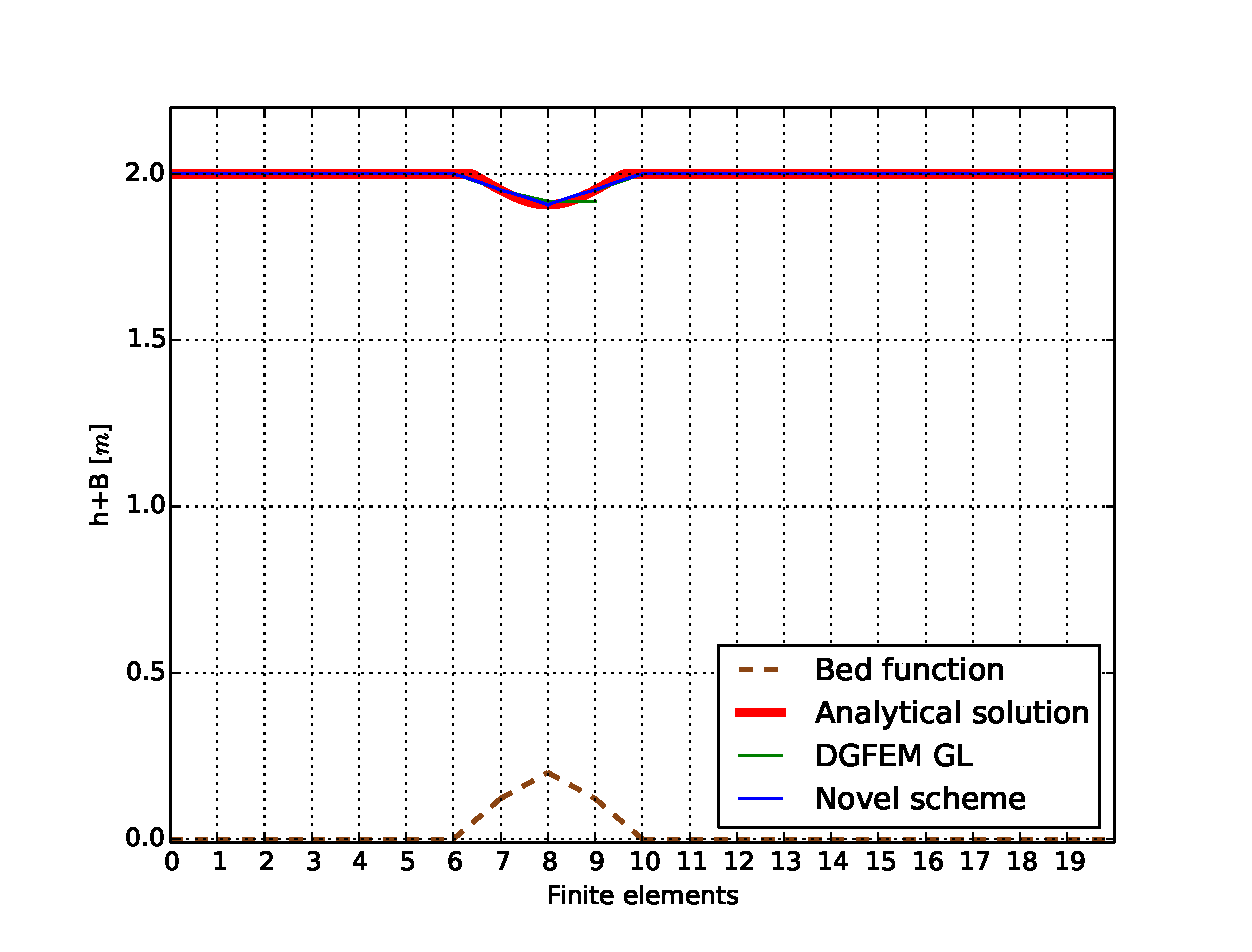
\includegraphics[width=1.0\textwidth]{OBR/bump/subH.eps}
								    \caption{Water depth: subcritical flow.}
								    \label{subH}
								    \end{center}
								\end{minipage}\hspace{15mm}
								\begin{minipage}[t]{0.44\textwidth}
								    \begin{center}
								    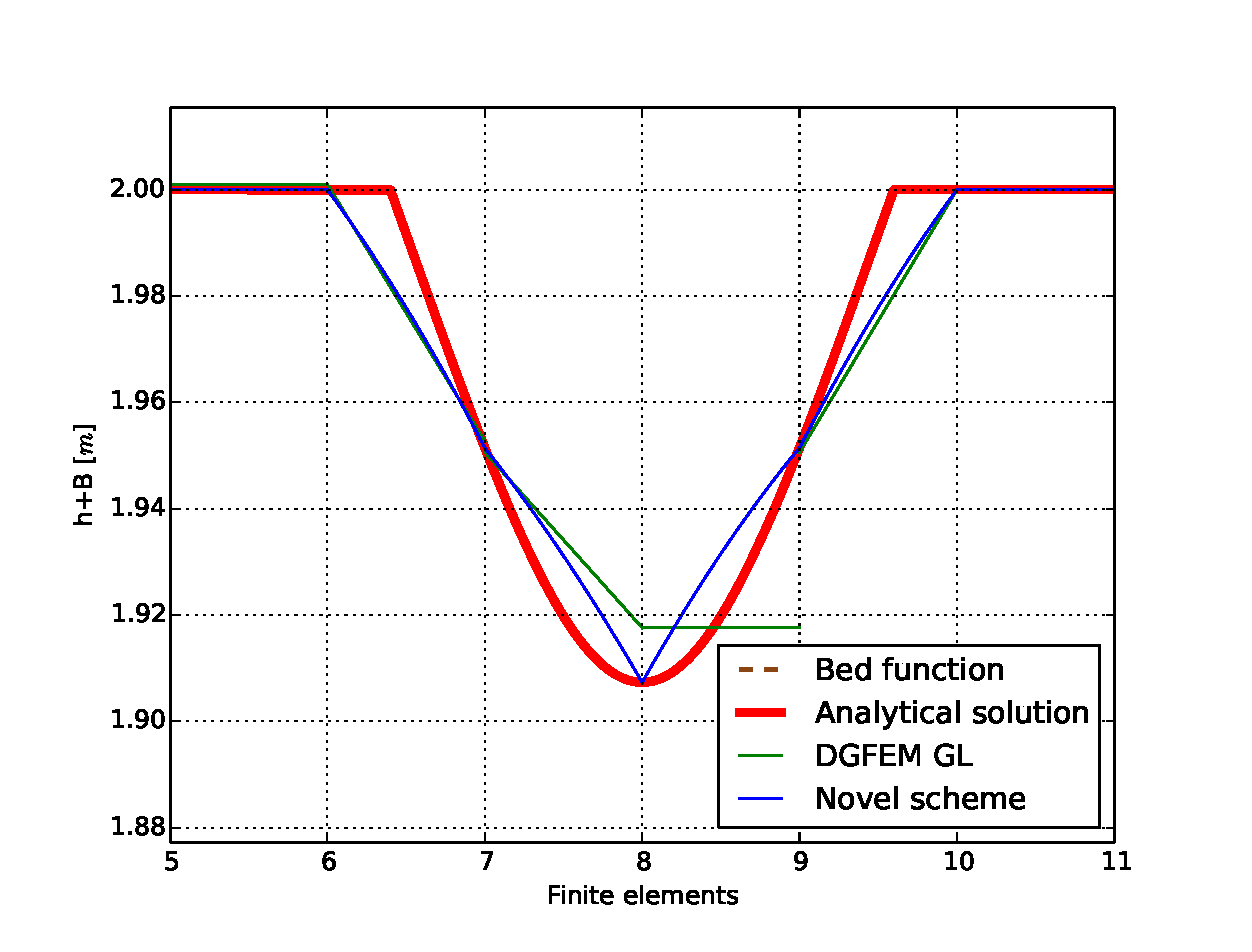
\includegraphics[width=1.0\textwidth]{OBR/bump/subHdet.eps}
								    \caption{Detail of the water depth: subcritical flow.}
								    \label{subHdet}
								    \end{center}
								\end{minipage}
				\end{figure}
				\begin{figure}[!ht]
								\centering
								 \begin{minipage}[t]{0.44\textwidth}
								    \begin{center}
								    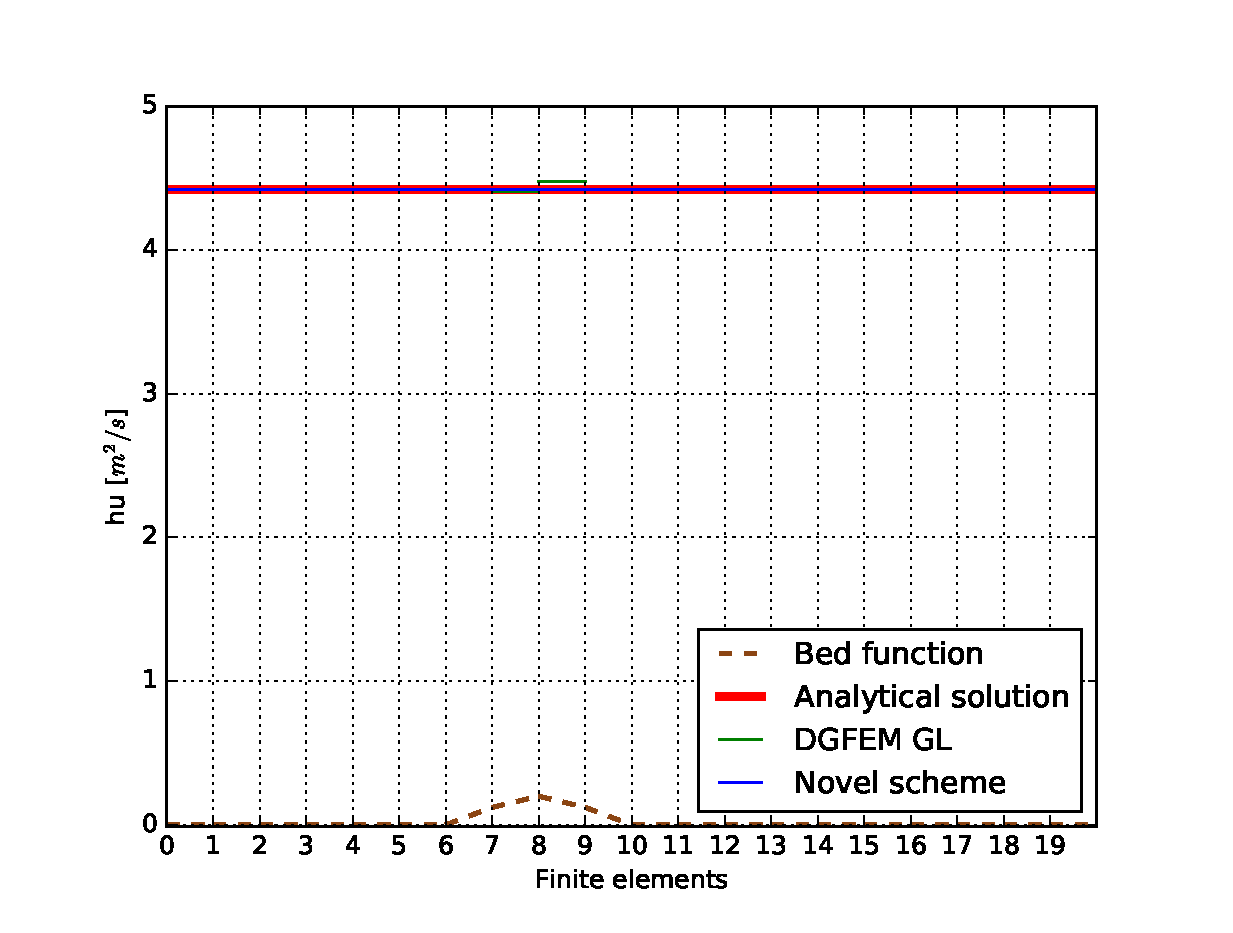
\includegraphics[width=1.0\textwidth]{OBR/bump/subHU.eps}
								    \caption{Discharge: subcritical flow.}
								    \label{subHU}
								    \end{center}
								\end{minipage}\hspace{15mm}
								\begin{minipage}[t]{0.44\textwidth}
								    \begin{center}
								    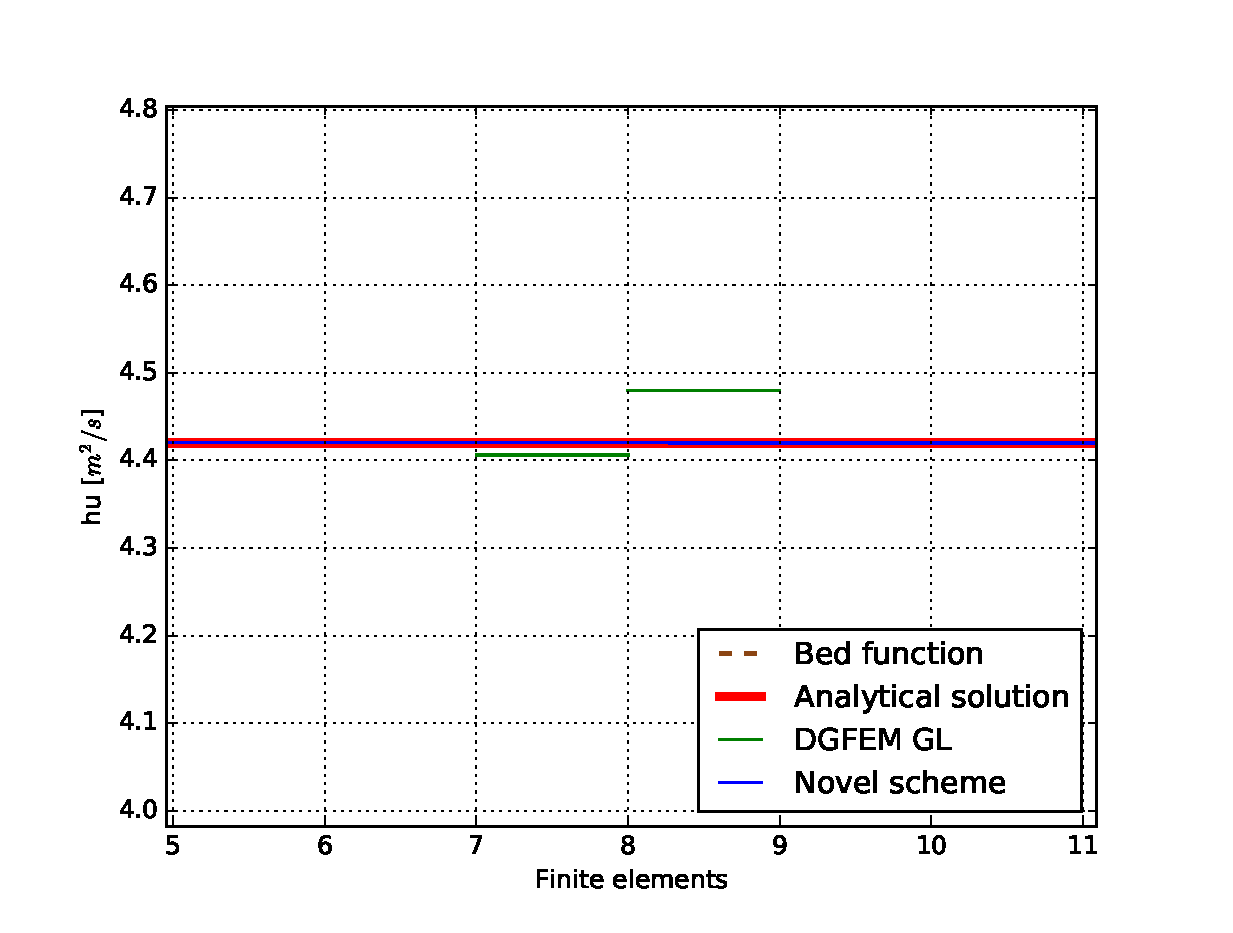
\includegraphics[width=1.0\textwidth]{OBR/bump/subHUdet.eps}
								    \caption{Detail of the discharge: subcritical flow.}
								    \label{subHUdet}
								    \end{center}
								\end{minipage}
				\end{figure}
The water depth is shown in Figure \ref{subH} and in Figure \ref{subHU} the discharge is shown. Details of the water depth and discharge can be seen in Figures \ref{subHdet} and \ref{subHUdet}. 

The boundary conditions of the transcritical flow without shock are 
\begin{equation}
\begin{array}{c}
q_{inlet}=1.53 \ m^2/s,\\
h_{outlet}=0.66 \ m
\end{array}
\end{equation}
and the analytical solution is given by the resolution of
\begin{equation}
h^3(x)+\left( B(x)-\frac{\text{q} _{inlet}^2}{2g \text{h}_M^2}-h_M-B_M \right) h^2(x)+\frac{\text{q} ^2_{inlet}}{2 g}=0, \quad \forall x \in [0,L]
\end{equation}
where $B_M=\text{max}_{x\in [0,L]}B(x)$ and $\text{h}_M$ is the corresponding water depth.
				\begin{figure}[!ht]
								\centering
								 \begin{minipage}[t]{0.44\textwidth}
								    \begin{center}
								    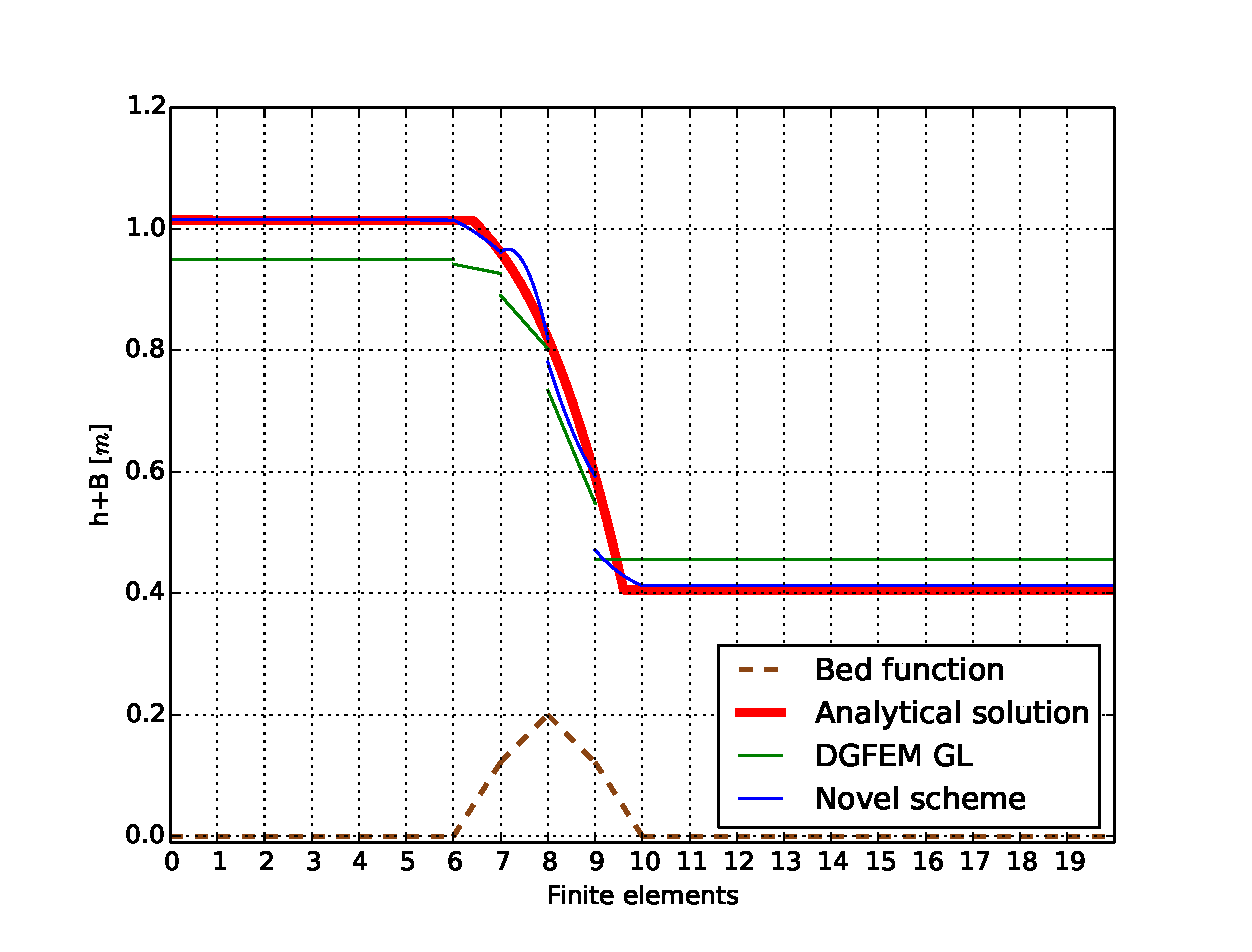
\includegraphics[width=1.0\textwidth]{OBR/bump/transH.eps}
								    \caption{Water depth: transcritical flow without the shock.}
								    \label{transH}
								    \end{center}
								\end{minipage}\hspace{15mm}
								\begin{minipage}[t]{0.44\textwidth}
								    \begin{center}
								    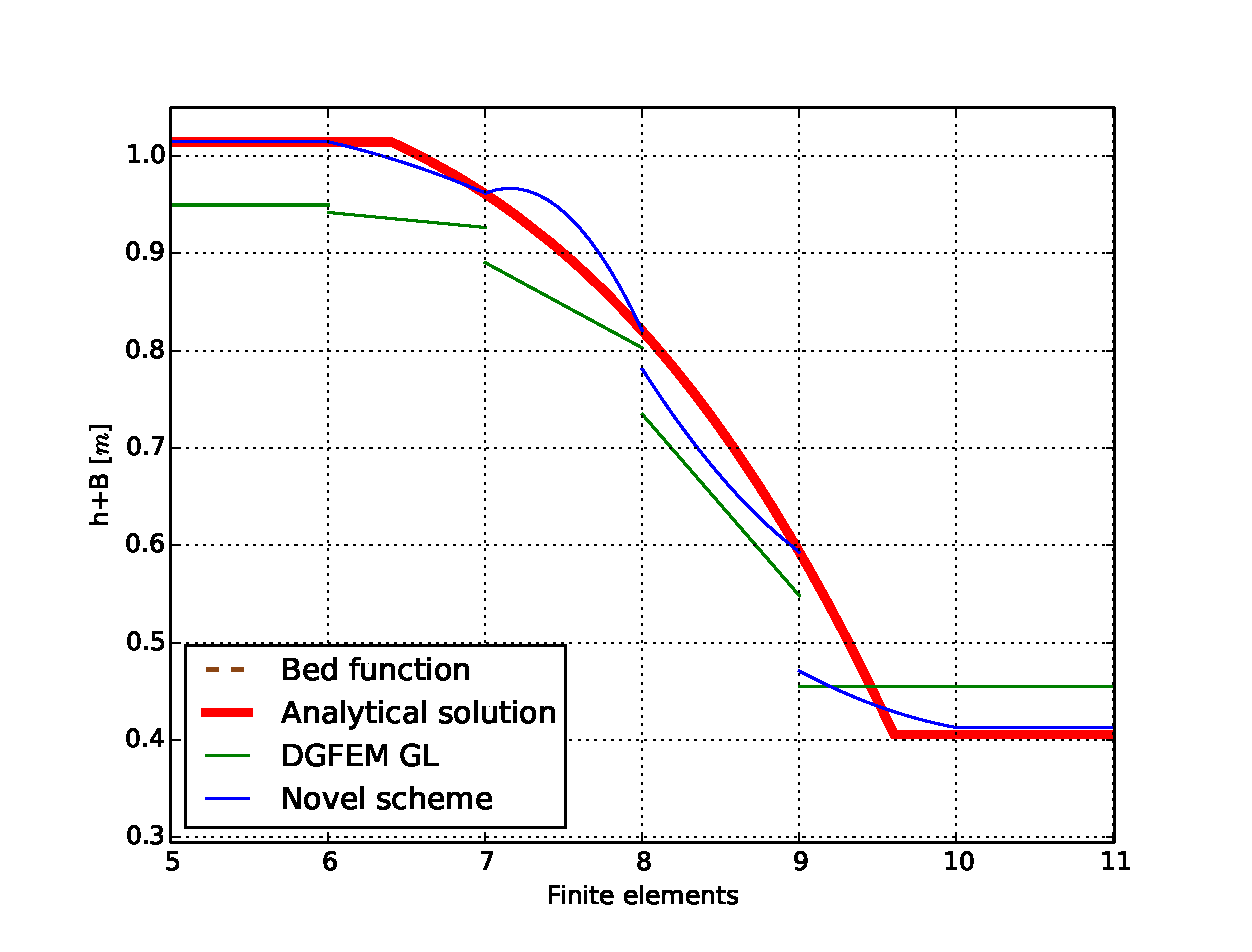
\includegraphics[width=1.0\textwidth]{OBR/bump/transHdet.eps}
								    \caption{Detail of the water depth: transcritical flow without the shock.}
								    \label{transHdet}
								    \end{center}
								\end{minipage}
				\end{figure}
								\begin{figure}[!ht]
								\centering
								 \begin{minipage}[t]{0.44\textwidth}
								    \begin{center}
								    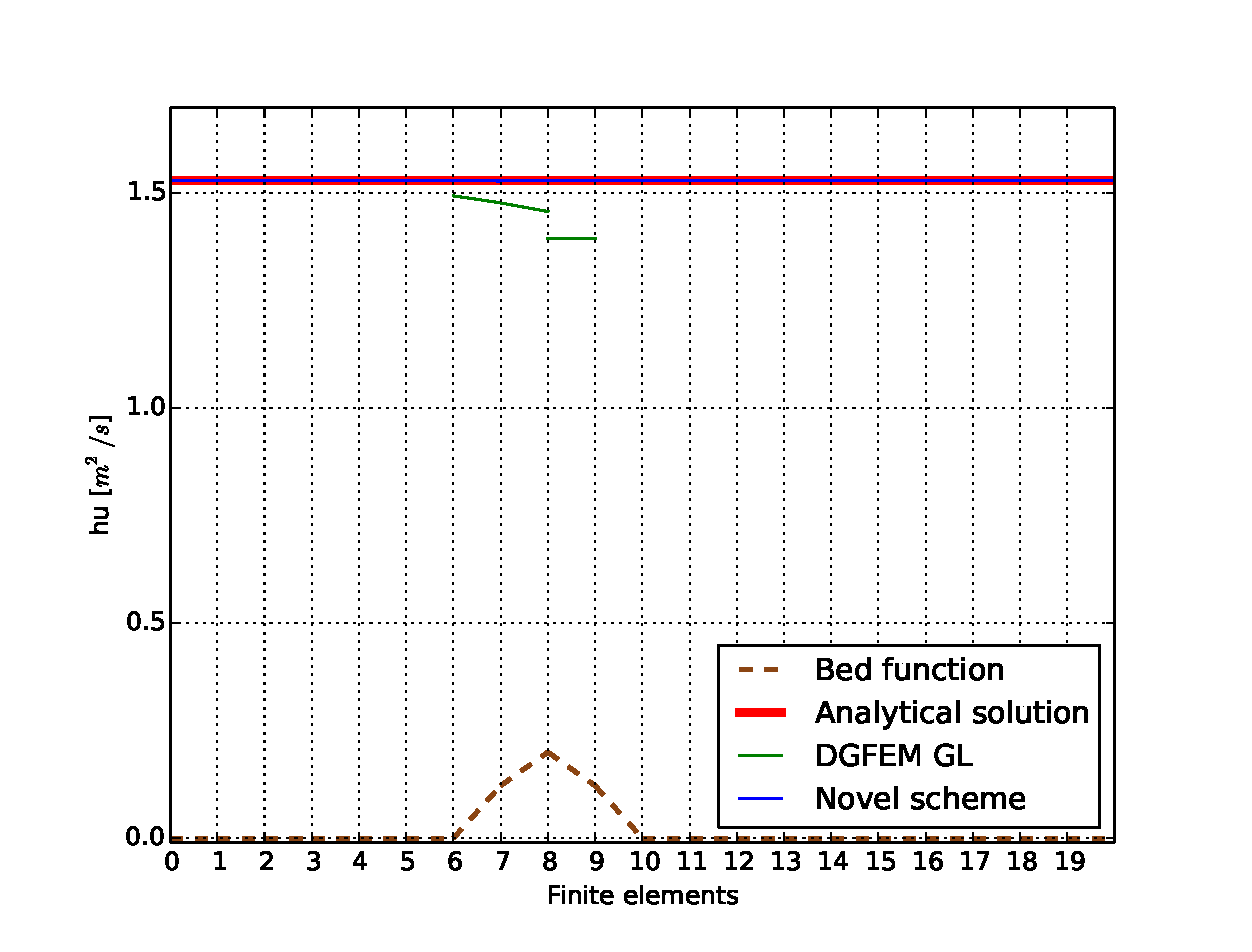
\includegraphics[width=1.0\textwidth]{OBR/bump/transHU.eps}
								    \caption{Discharge: transcritical flow without the shock.}
								    \label{transHU}
								    \end{center}
								\end{minipage}\hspace{15mm}
								\begin{minipage}[t]{0.44\textwidth}
								    \begin{center}
								    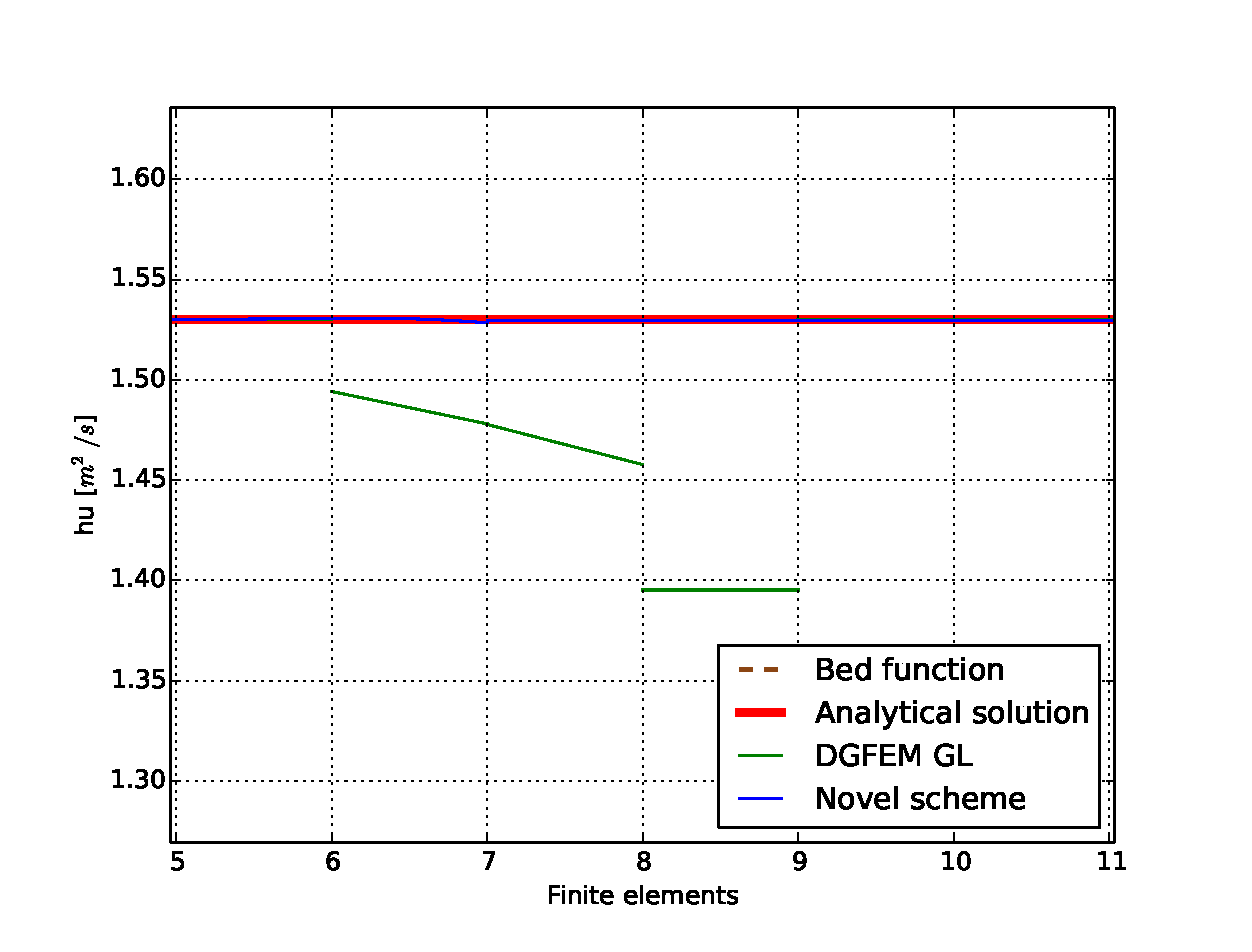
\includegraphics[width=1.0\textwidth]{OBR/bump/transHUdet.eps}
								    \caption{Detail of the discharge: transcritical flow without the shock.}
								    \label{transHUdet}
								    \end{center}
								\end{minipage}
				\end{figure}
In Figures \ref{transH} and \ref{transHdet} the water depth can be seen and the discharge can be seen in Figures \ref{transHU} and \ref{transHUdet}.

Boundary conditions of the transcritical flow with shock are given by 
\begin{equation}
\begin{array}{c}
q_{inlet}=0.18 \ m^2/s,\\
h_{outlet}=0.33 \ m.
\end{array}
\end{equation}
and the analytical solution is given by the resolution of
\begin{equation}\label{desitkaSwa}
\begin{array}{r}
h^3(x _{shock})+\left( B(x _{shock})-\frac{\text{q} ^2_{inlet} }{2g \text{h}^2_M}-\text{h}_M-B_M \right)h^2(x_{shock})+\frac{\text{q} ^2_{inlet}}{2g}=0,\\

h^3(x _{shock})+\left( B(x _{shock})-\frac{\text{q} ^2_{inlet} }{2g \text{h}^2_{outlet}}-\text{h}_{outlet} \right)h^2(x_{shock})+\frac{\text{q} ^2_{inlet}}{2g}=0,\\
\text{q} ^2_{inlet}\left(\frac{1}{h_1}-\frac{1}{h_2}\right)+\frac{g}{2}(h_1^2-h_2^2)=0
\end{array}
\end{equation}
where $h_1$ and $h_2$ are the water depths upstream and downstream respectively. The position of the shock $x_{shock}$ is located thanks to the third relation in system (\ref{desitkaSwa}) which is known as Rankine-Hugoniot’s relation. The reader is referred to \cite{noelle} to see the details.
				\begin{figure}[!ht]
								\centering
								 \begin{minipage}[t]{0.44\textwidth}
								    \begin{center}
								    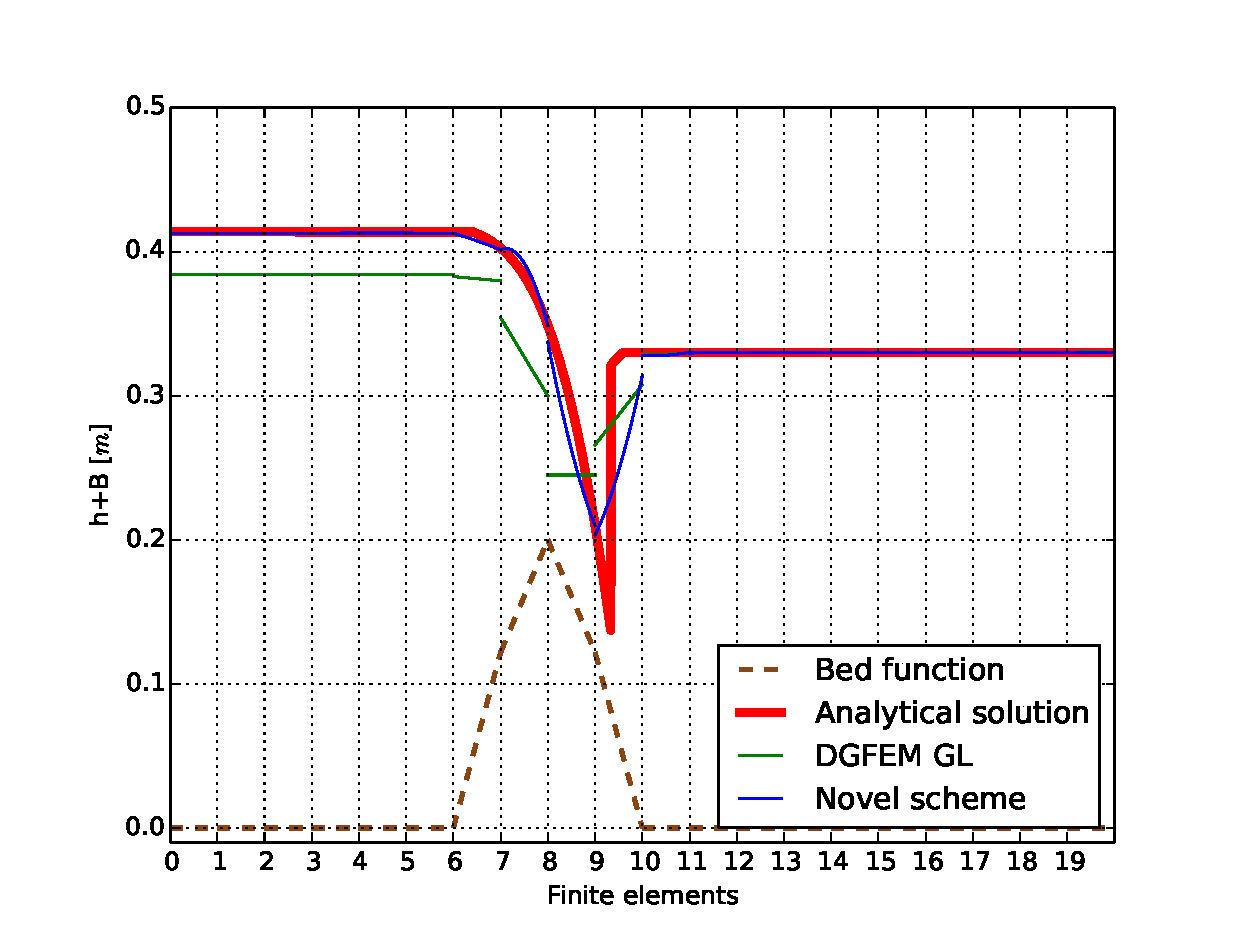
\includegraphics[width=1.0\textwidth]{OBR/bump/shockH.eps}
								    \caption{Water depth: transcritical flow with the shock.}
								    \label{shockH}
								    \end{center}
								\end{minipage}\hspace{15mm}
								\begin{minipage}[t]{0.44\textwidth}
								    \begin{center}
								    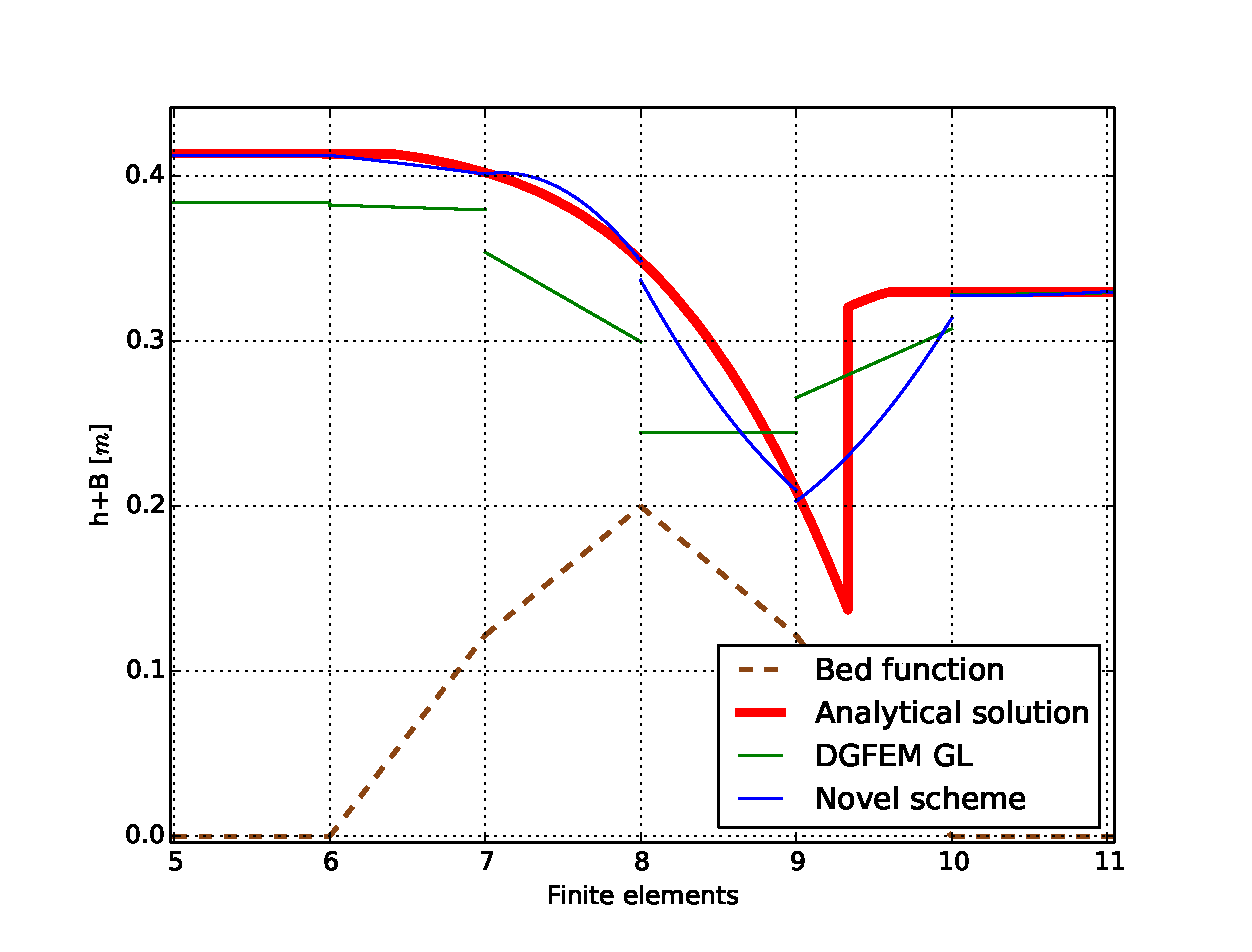
\includegraphics[width=1.0\textwidth]{OBR/bump/shockHdet.eps}
								    \caption{Detail of the water depth: transcritical flow with the shock.}
								    \label{shockHdet}
								    \end{center}
								\end{minipage}
				\end{figure}
								\begin{figure}[!ht]
								\centering
								 \begin{minipage}[t]{0.44\textwidth}
								    \begin{center}
								    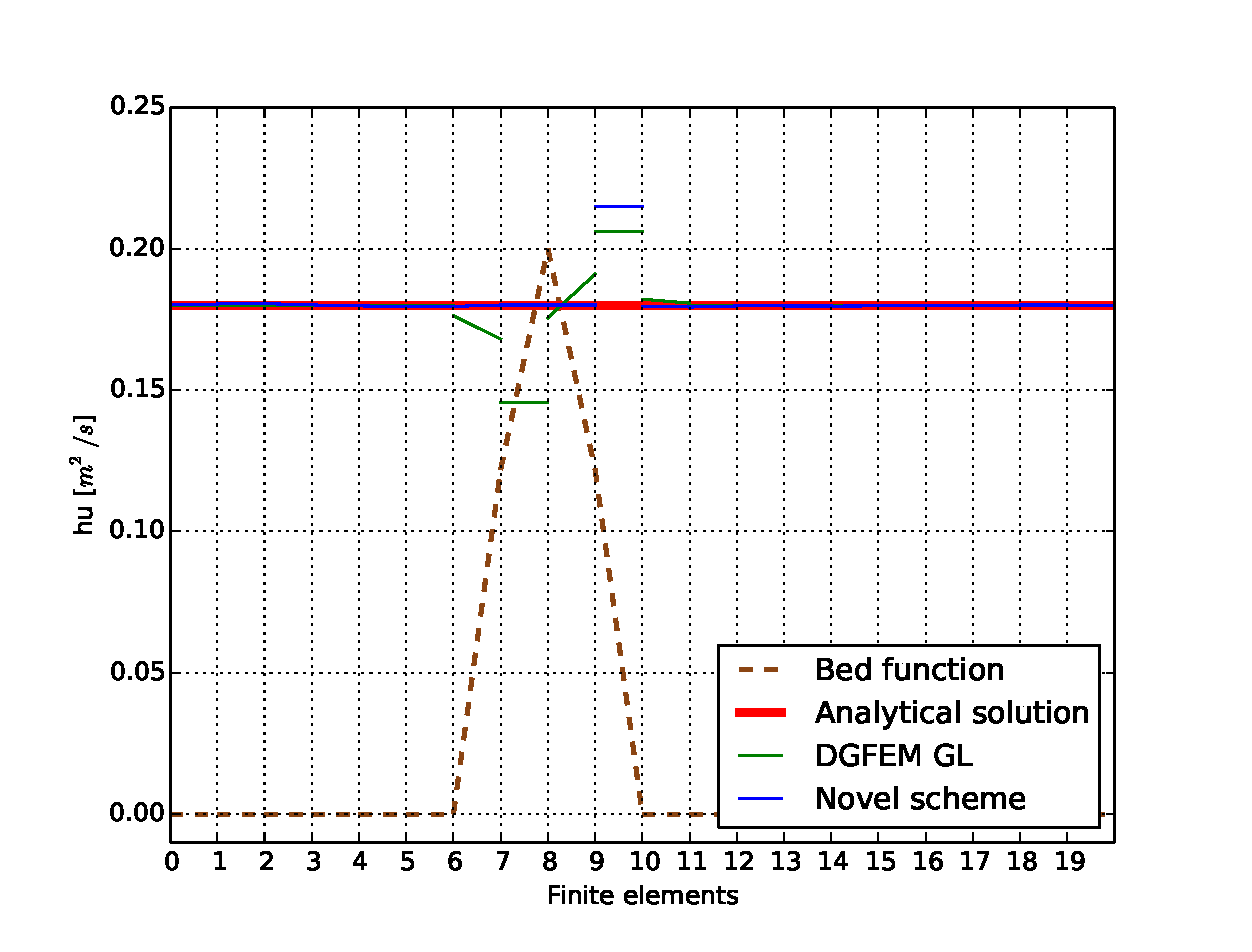
\includegraphics[width=1.0\textwidth]{OBR/bump/shockHU.eps}
								    \caption{Discharge: transcritical flow with the shock.}
								    \label{shockHU}
								    \end{center}
								\end{minipage}\hspace{15mm}
								\begin{minipage}[t]{0.44\textwidth}
								    \begin{center}
								    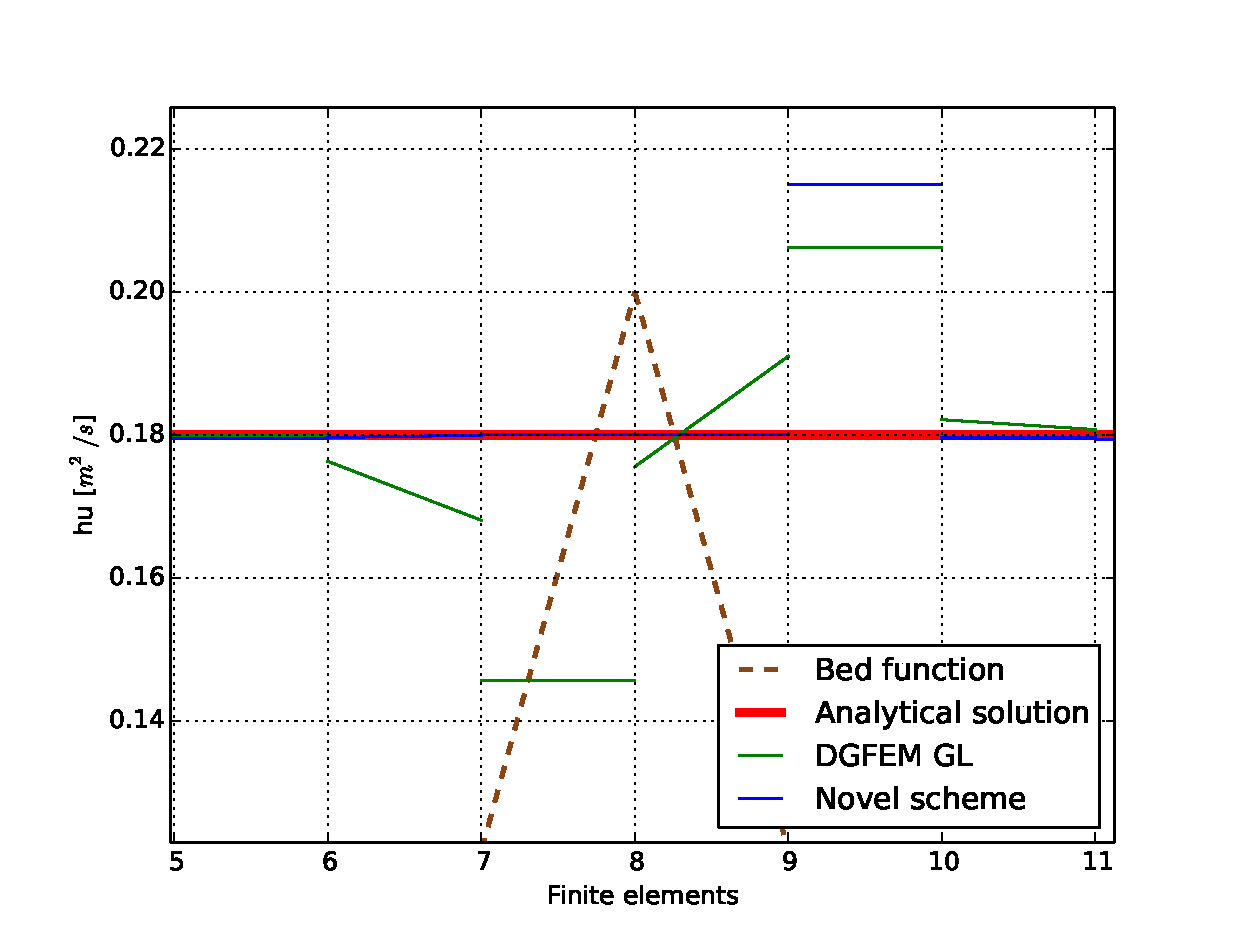
\includegraphics[width=1.0\textwidth]{OBR/bump/shockHUdet.eps}
								    \caption{Detail of the discharge: transcritical flow with the shock.}
								    \label{shockHUdet}
								    \end{center}
								\end{minipage}
				\end{figure}
Numerical solution of the water depth is shown in Figures \ref{shockH} and \ref{shockHdet}. In Figures \ref{shockHU} and \ref{shockHUdet} the discharge is shown.
\section{Conclusion}

Novel limiting criterion for limiting process within discontinuous Galerkin method was introduced. This criterion works for both water depth and discharge variables. In Section \ref{DBwet} and \ref{psp}, there was proven that this novel numerical scheme brings better accuracy than finite volume method and DGFEM with global limiting. In the paper there is also successfully implemented the wet/dry treatment used in the theory of finite volumes. This treatment ensures non-negativity of the water depth. Adopted velocity modification (\ref{formVel}) avoids appearance of the non-physically large velocities caused by numerical inaccuracy.



It is concluded that the presented scheme is able to solve the flow over complex topography and keep the C-property in the flooded domain. The scheme also give good results for both wetting and drying processes.

 The future work can be focused on the bed friction source term and its stability around wet/dry interface when the water depth is approaching zero values and wet/dry interface treatment for the bed function described by higher order polynomials.
\section*{Acknowledgment}


\bibliography{library}{}
%\bibliographystyle{plain}%plain unsrt
\end{document}

